% Chapter 1

\chapter{Instruments descriptions} % Main chapter title

\label{Chapter3} % For referencing the chapter elsewhere, use \ref{Chapter1} 



%----------------------------------------------------------------------------------------

\section{Layout of Photon calibrator}
The KAGRA photon calibrator is placed around EXA/EYA chamber, which is installed 36 m away from the end test mass (ETM). We push the mirror surface with the modulated photon pressure directly. Figure \ref{fig:Pcal_overview} shows the layout of the KAGRA photon calibrator. The photon calibrator consists of transmitter module (Tx module), receiver module (Rx module), periscope, and telephoto camera module (TCam module). We place the 20~W laser in Tx module, whose frequency is 1047 nm. The 1064 nm laser is not used due to avoid the coupling with main beams.   The power of the laser is modulated by the optical follower servo (OFS). We split the beams in Tx module for pushing the drum head node points of the ETM due to elastic deformation. We transfer the beams to the ETM though the periscope. All the periscope structures are placed into the EXA/EYA chamber. The beam is received by the Rx module. We place a 6 inches integrating sphere for the accurate measurement of the laser power and two quadrant photo detector (QPD) for the beam position monitor. We also measure the beam position on the ETM surface using the telephoto camera (TCam). The Tcam is consists of the astronomical telescope, focuser, and high resolution digital camera. The specification summary of KAGRA photon calibrator is shown in Tabel.~\ref{tab:KAGRA_spec}. Details of instruments are described following section.
\begin{figure}
\begin{center}
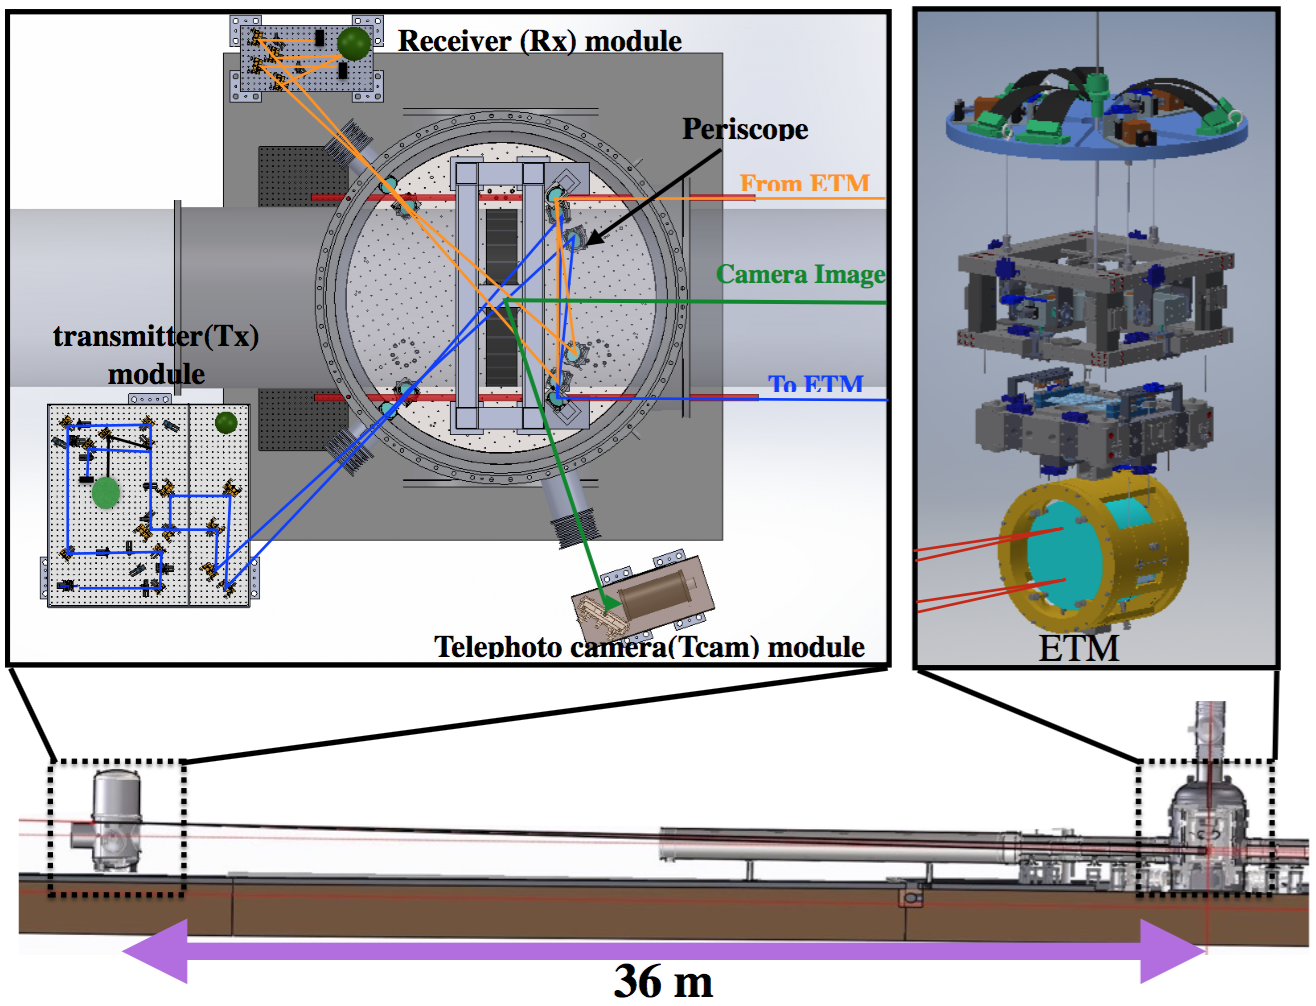
\includegraphics[width=15cm]{Figures/Pcal_overview.eps}
\caption{KAGRA photon calibrator. The calibration system is placed around the EXA/EYA chamber. We mount the optical lever and optical baffle as well. The EXA/EYA chambers are placed at 36 m far from the ETM.} 
\label{fig:Pcal_overview} 
\end{center}
\end{figure}

\begin{table}
\caption{Specification summary of photon calibrator.}
\label{tab:KAGRA_spec}
\centering
\begin{tabular}{cccc}
\toprule
\tabhead{} & \tabhead{KAGRA} & \tabhead{advanced LIGO} & \tabhead{advanced Virgo} \\
\midrule
 Mirror material & Sapphire & Silica & Silica \\
 Mirror mass & 22.8 kg & 42 kg & 40 kg \\
  Mirror diameter & 220 mm & 340 mm & 350 mm \\
    Mirror thickness & 150 mm & 200 mm & 200 mm \\
 Distance of Pcal from ETM & 36 m & 8 m & 1.5 m \\
  Pcal laser power & 20 W & 2W & 3 W \\
  Laser frequency & 1047 nm & 1047 nm &1047 nm\\
  Incident angle& 0.72 deg & 8.75 deg &30 deg \\
\bottomrule\\
\end{tabular}
\end{table}
%----------------------------------------------------------------------------------------

\section{Transmitter (Tx) module}
The Tx module is placed at the side of the EXA/EYA chamber. Figure~\ref{fig:Tx_module_overview} shows the view of Transmitter module. All the optical components are mounted on the $900~\mathrm{mm}\times  900~\mathrm{mm}$ breadboard (B9090L; Thorlabs). The bread board is placed on the support structure. The electrical module for the control and readout are also hosed in the support structure. 

\begin{figure}
\begin{center}
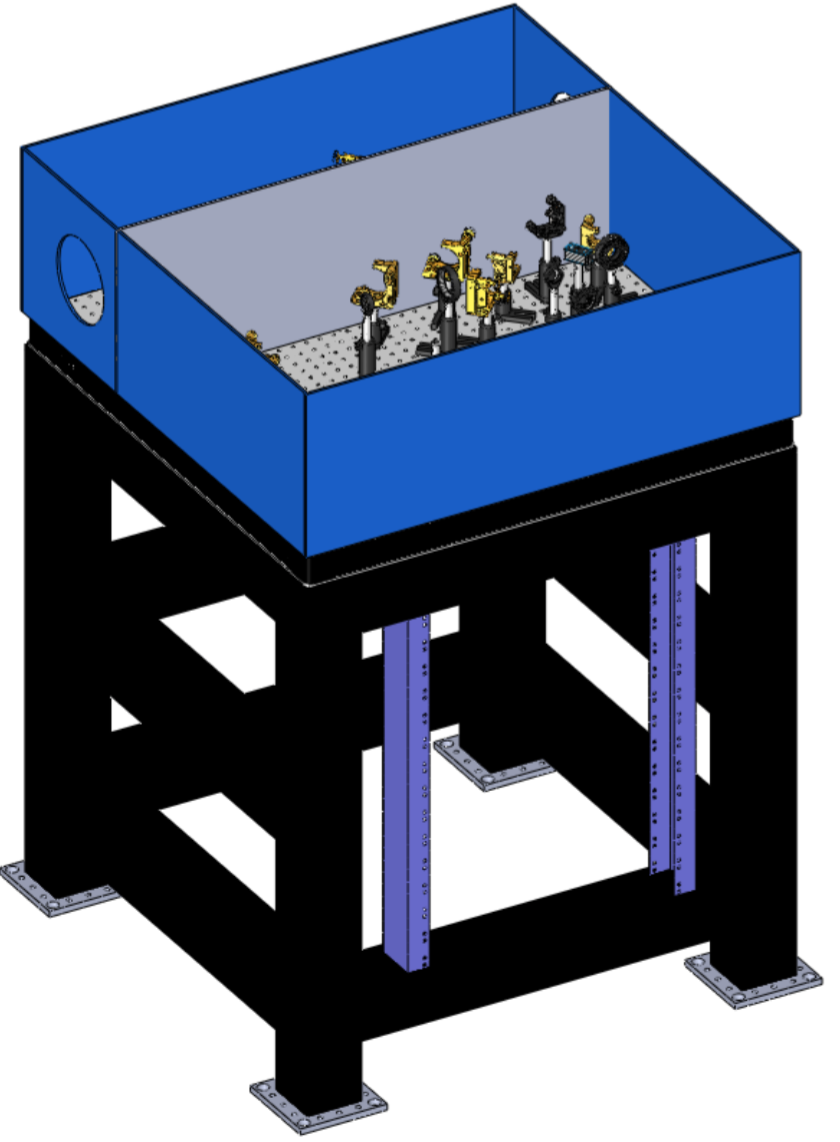
\includegraphics[width=12cm]{Figures/Tx_module_overview.eps}
\caption{Transmitter module of KAGRA Pcal. We place the optical table on the triangle table. The readout and control device are housed into the legs of table.} 
\label{fig:Tx_module_overview} 
\end{center}
\end{figure}

Figure~\ref{fig:Tx_module_layout} shows the optical layout of Tx module.

\begin{figure}
\begin{center}
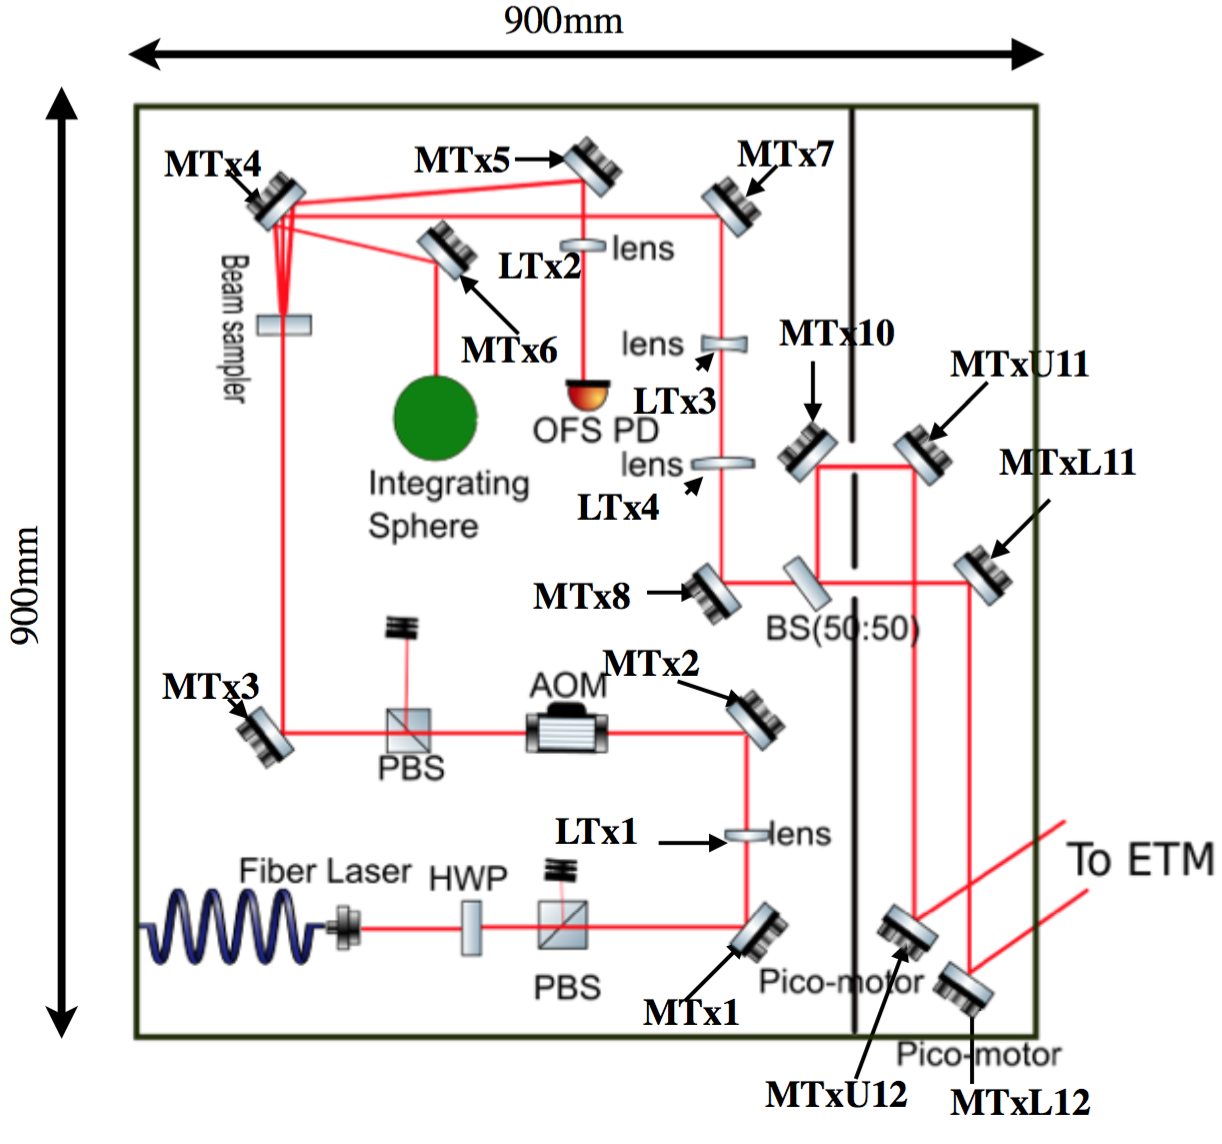
\includegraphics[width=12cm]{Figures/Tx_module_layout.eps}
\caption{Optical layout of KAGRA photon calibrator. The laser power is modulated and controlled by the acousto-optic modulator (AOM). This modulated laser is sent to a 50:50 beam splitter, where we monitor the modulated laser power by using the integrating sphere.} 
\label{fig:Tx_module_layout} 
\end{center}
\end{figure}

\subsection{Fiber laser}
We employ the CW fiber laser made by the LER photonics as shown in Fig.~\ref{fig:Laser}. The maximum power and frequency are 20 W and 1047 nm, respectively. The model number of the laser is CYFL-TERA-20-LP-1047-AM1-RGO-OM1-T305-C1. The maximum laser power of KAGRA Pcal is 10 times larger than that of LIGO. This is because that we need the high power laser for the injection test and photon pressure actuator technique. The typical beam width of the laser is 0.25~mm when we mount the isolator. We summarize the specification of the laser as shown in Table~\ref{tab:Laser_spec}.

\begin{figure}
\begin{center}
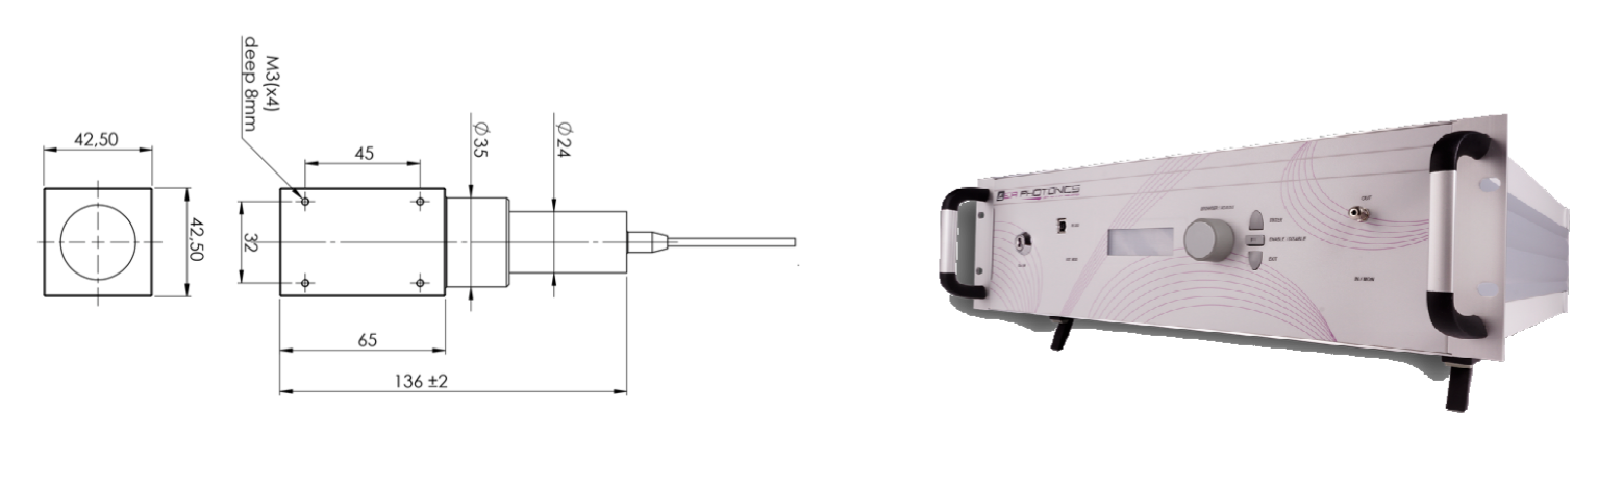
\includegraphics[width=14cm]{Figures/Laser.eps}
\caption{The fiber laser and drawing of isolator. The module is placed under the Tx module.} 
\label{fig:Laser} 
\end{center}
\end{figure}

\begin{table}
\caption{Specification summary of CW fiber Laser.}
\label{tab:Laser_spec}
\centering
\begin{tabular}{ ccccc}
\toprule
\tabhead{Charactaristic} & \tabhead{Typical value} & \tabhead{Unit} & \tabhead{Note} \\
\midrule
Operating central wavelength & 1047 & nm & $\pm1~\mathrm{nm}$\\
CW output power & 20 & W & \\
Output signal line-width & 0.5 & nm & FWHM\\
Output power stability & $\pm1$&\%RMS& Output power: 20~W\\
Output power tunability & 10-100&\%& \\
Optical polarization & Linier&& \\
Polarization extinction ratio & 15&dB& \\
Output fiber & PLMAFUD3460&& Nufurn company \\ 
Output fiber length & 2&m&  \\
Beam diameter & 0.5&mm& with isolator  \\
Beam quality & 1.1&$M^2$&   \\
Control & Active current control,&&   \\
mode & Active power control&&   \\
Beam quality & 1.1&$M^2$&     \\
Supply voltage & 84-264&V&AC 47 to 63 Hz   \\
Power consumption & 650&W&   \\
Housing & 448x451x132.5&mm&   \\
Total weight & 13&kg&   \\
Cooling & Air cooled with fans&&   \\
Operating temperature & 15-35&&   \\
Humidity & 5-85&\%&   \\
\bottomrule\\
\end{tabular}
\end{table}

\subsection{Beam shutter}
We have to pay attention to safety for the operation of the high power laser. In order to dump the beam, we use the beam shutter made by lasermet company. The model number of the shutter is LS-10-12. The aperture size and  maximum laser power are 15 mm and 20 W. These number meet our requirement due to the laser spot size and maximum power. We control the beam shutter on the MEDM as shown in Sec.~\ref{MEDM}. The specification of the beam shutter is shown in Table.~\ref{tab:Beam_shutter_spec}.

\begin{table}
\caption{Specification of beam shutter.}
\label{tab:Beam_shutter_spec}
\centering
\begin{tabular}{ ccccc}
\toprule
\tabhead{Charactaristic} & \tabhead{Typical value} & \tabhead{Unit} & \tabhead{Note} \\
\midrule
Max laser power & 20 & W & \\
Aperture size & 15 & mm & \\
Drive voltage & 11-14 & V DC & \\
Current consumption & 150 & mA & \\
Size & $98 \times 63.5 \times 36$ & mm & \\
\bottomrule\\
\end{tabular}
\end{table}

\subsection{Zeroth order half wave plate}
To control the polarization angle of the incident beam, we employ the zeroth order half wave plate (HWP) made by the CVI laser optics. The model number of the HWP is QWPO-1047-05-2-R10 whose diameter is 12.7 mm. The HWP is mounted on the rotation mount made by Thorlabs. The thickness are optimized at 1047 nm.
The specification of the HWP is listed in Table~\ref{tab:HWP_spec}.
\begin{table}
\caption{Specification of HWP.}
\label{tab:HWP_spec}
\centering
\begin{tabular}{ ccccc}
\toprule
\tabhead{Charactaristic} & \tabhead{Typical value} & \tabhead{Unit} & \tabhead{Note} \\
\midrule
Waveplate Type & Quartz Waveplates &  & \\
Wavelength Range & 1047 & nm & \\
Retardance & $\lambda/2$&  & \\
Clear Aperture & 85 & \% & of diameter \\
Reflection & 0.25 & \% & \\
Retardance Tolerance & $\lambda/200$ to $\lambda/500$ & & at 23Degree C \\ %% SH Please avoid using unicode
Material & Crystal Quartz &  & \\
Surface Quality & 10-5  & scratch-dig & \\
Waveplate Diameter & 12.7 & mm & \\
\bottomrule\\
\end{tabular}
\end{table}

\subsection{Polarizer}
We place two polarizers to define the polarization angle accurately. This is because that the power of the laser is modulated by acousto-optic modulator (AOM) whose performance depend on the incident polarization angle.
One polarizer is placed behind HWP. Another one is placed after AOM. The polarizer is made by Karl-Lambrecht. We purchased TFPC12-1047 that is optimized at 1047 nm. 

\subsection{Lens}
We have dane a mode matching simulation using JamMt. We assumed laser beam to be gaussian distribution. We have to place the focus of the laser at the AOM. Thus, we decide the optimal position and focal length of the 1 inch lens (LTx1), where the assumed beam waist of the fiber laser and AOM are 0.25 mm, respectively. The estimated beam spot size and lens position are shown in Fig.~\ref{fig:Mode_L1}.
\begin{figure}
\begin{center}
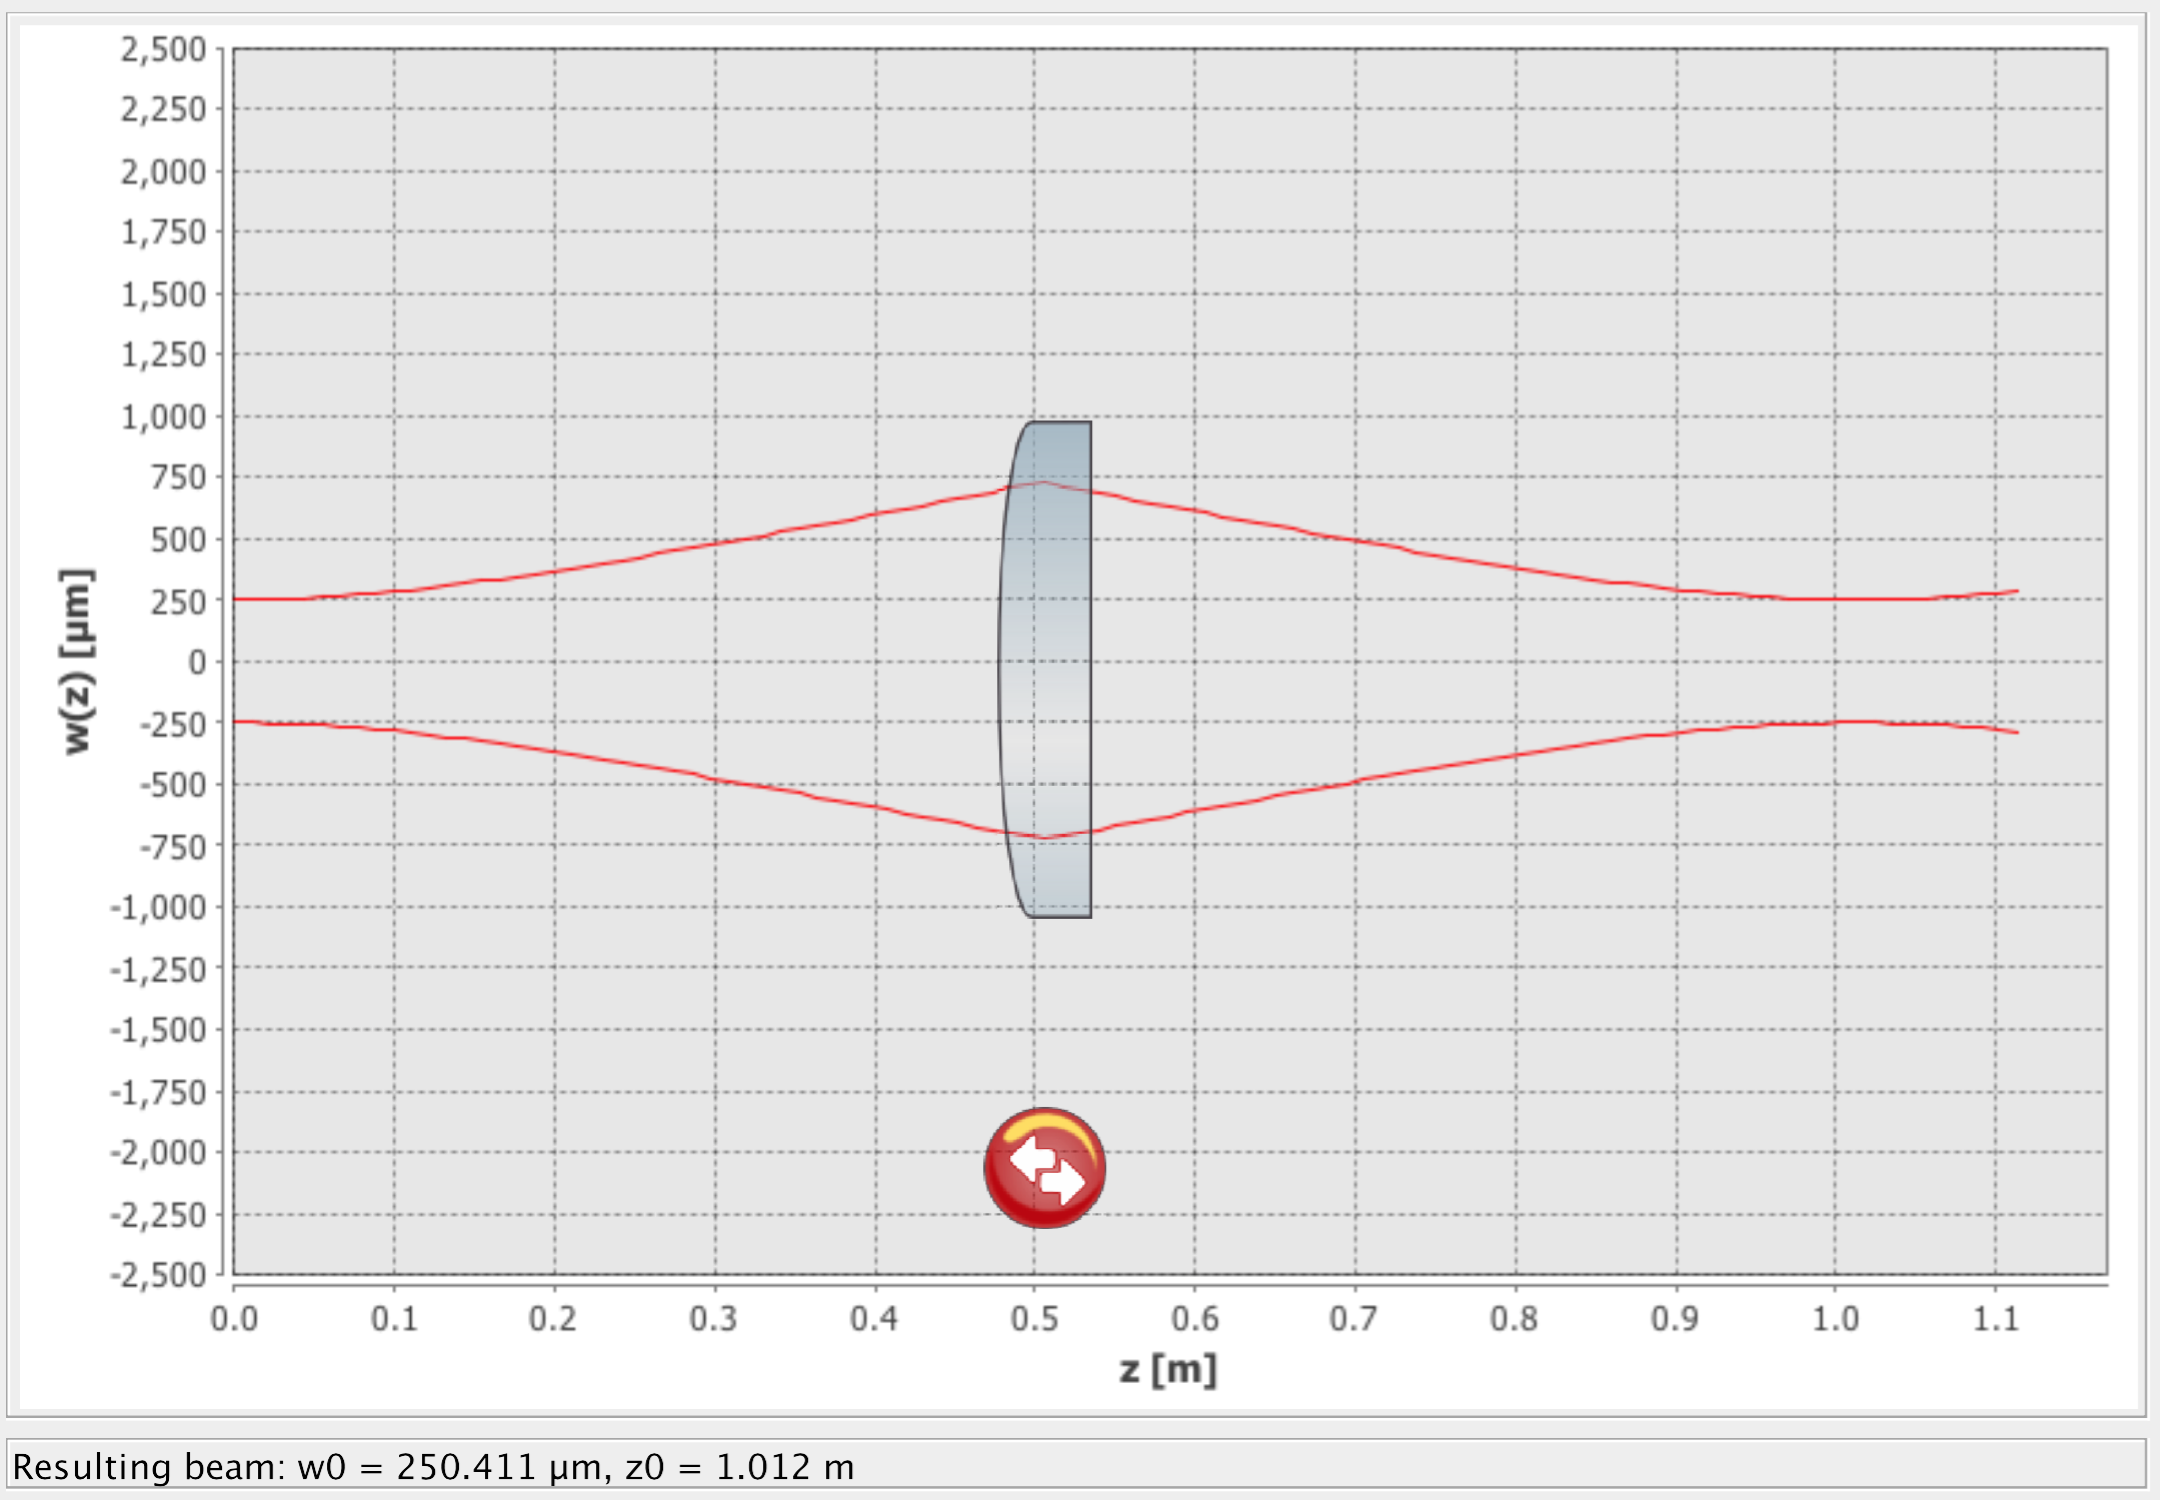
\includegraphics[width=14cm]{Figures/Mode_L1.eps}
\caption{Result of mode matching calculation from faber laser to AOM focus using JamMt.} 
\label{fig:Mode_L1} 
\end{center}
\end{figure}

Furthermore, we place two lenses for placing the focus at the surface of the ETM. We employ the combination of 1 inch negative lens (LTx3) and 2 inch positive lens(LTx4). The Gaussian beam can describe the following relation:
\begin{equation}
w(z)=\omega_0\sqrt{1+\left( \frac{\lambda z}{\pi \omega_0^2}\right)^2},
\end{equation}
where $\lambda$ is wavelength of the laser, $w_0$ is beam waist, $z$ is direction from the focus. We estimate the minimum differential beam spot by changing beam waist because it make the alignment easier. The minimum beam spot is written by 
\begin{equation}
\left .\frac{dw(z)}{dw_0} \right|_{z=36~\mathrm{m}}=0.
\end{equation}
The estimated beam spot is 5.5 mm at Tx module with 3.5 mm beam waist as shown in Fig.~\ref{fig:Mode_L3L4}.
\begin{figure}
\begin{center}
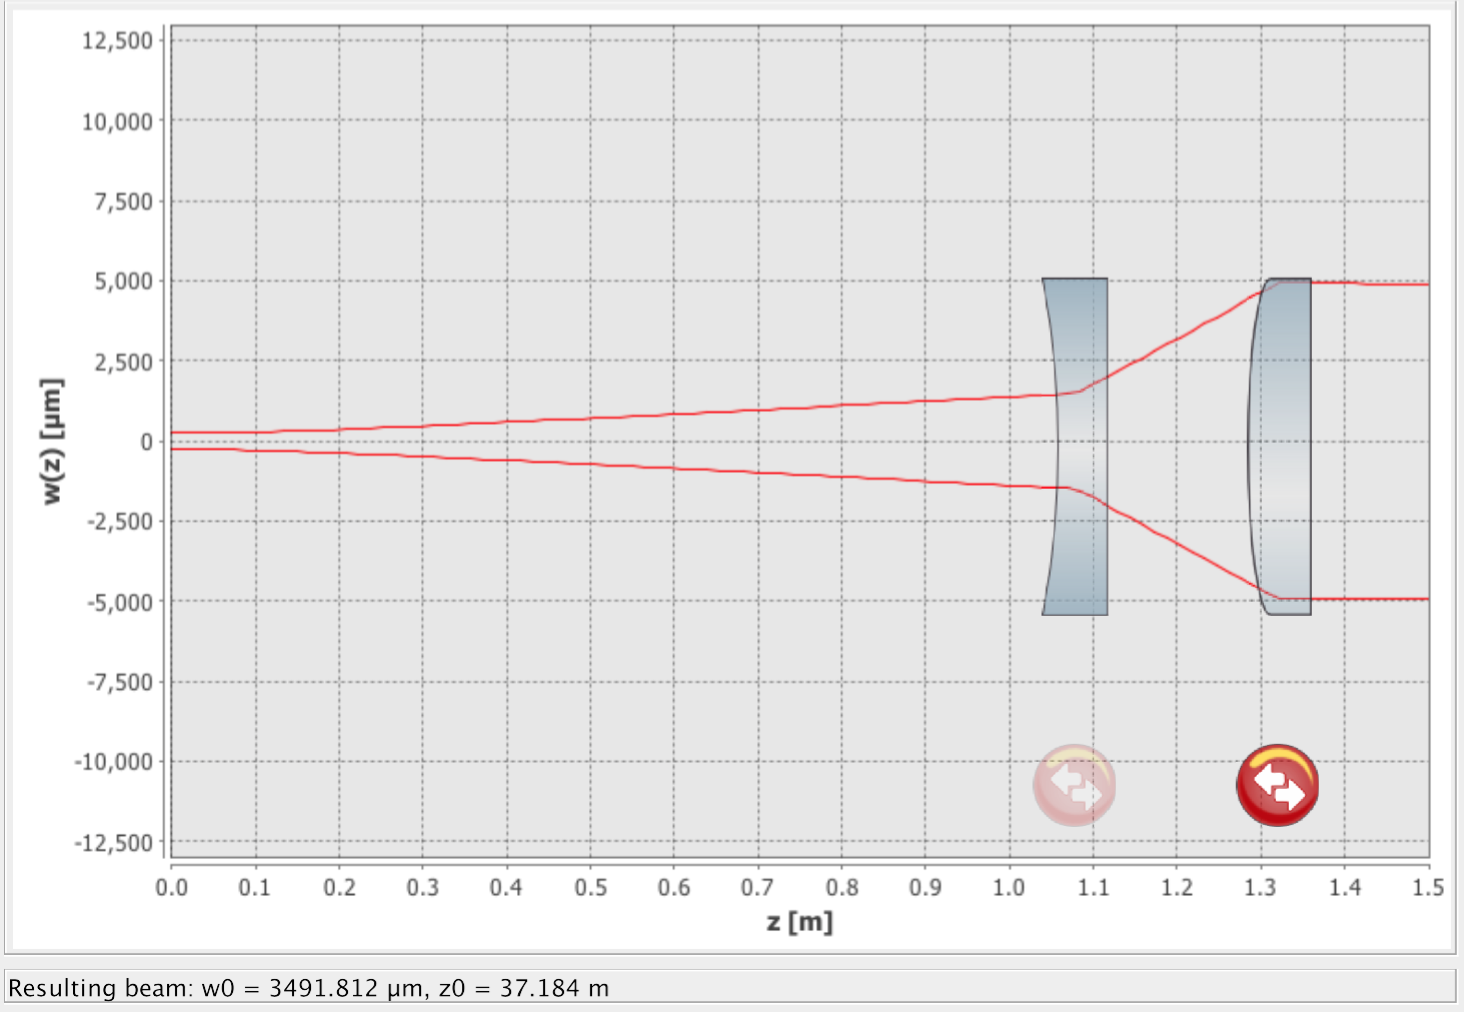
\includegraphics[width=14cm]{Figures/Mode_L3L4.eps}
\caption{Result of mode matching calculation from the AOM to the ETM focus using JamMt.} 
\label{fig:Mode_L3L4} 
\end{center}
\end{figure}

We also place the 1 inch lens (LTx2) at the front of the photo detector for the OFS.
The calculated spot size is shown in Fig.~\ref{fig:Mode_L2}. The beam width at the detector is $110~\mathrm{\mu m}$
\begin{figure}
\begin{center}
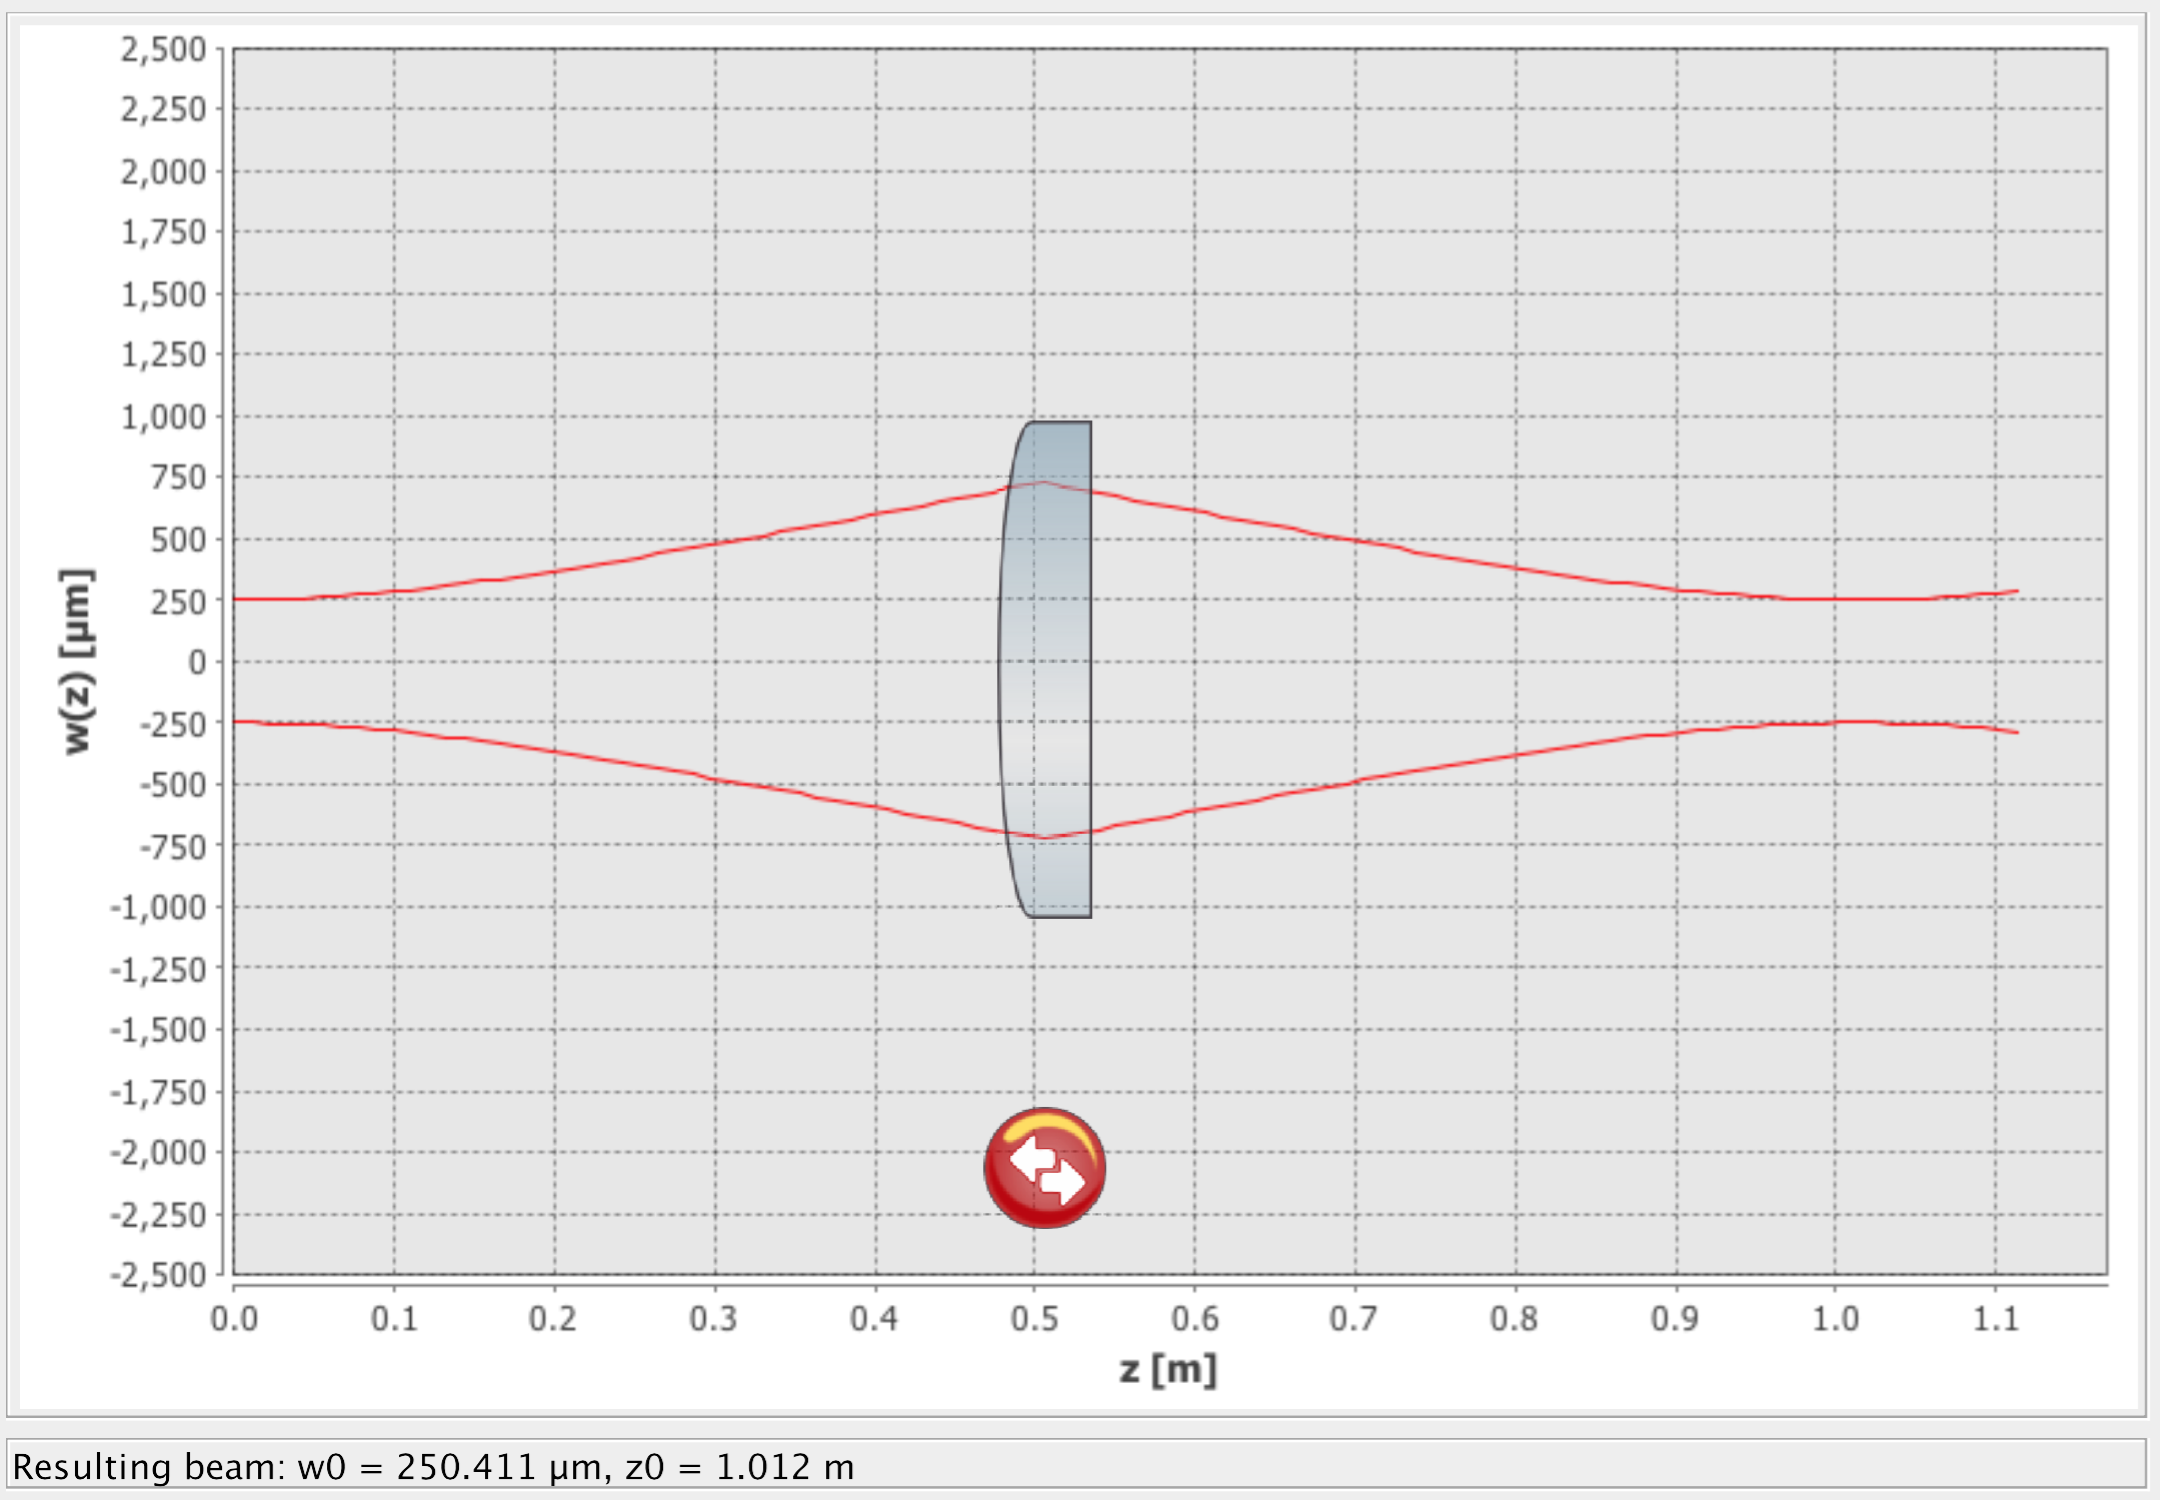
\includegraphics[width=14cm]{Figures/Mode_L1.eps}
\caption{Result of mode matching calculation from AOM to photo detector focus using JamMt.} 
\label{fig:Mode_L2} 
\end{center}
\end{figure}
 The parameters of the simulation results are listed in Table.~\ref{tab:Tx_lenses_spec}. All lenses are made by CVI laser optics. The material of lenses are fused silica. The AR coating are placed on both surface. 

\begin{table}
\caption{Specification of lenses.}
\label{tab:Tx_lenses_spec}
\centering
\begin{tabular}{ cccccc}
\toprule
\tabhead{Lens number} & \tabhead{part number}& \tabhead{Diameter [mm]} & \tabhead{Focal length (mm)} &\tabhead{z (mm)} &\tabhead{$w_0$ (mm)}   \\
\midrule
LTx1 &PLCX250UV (CVI laser optics) & 25.4 & 286.457&507&0.25\\
LTx2 &PLCX250UV (CVI laser optics)  & 25.4& 286.457 &507&0.25\\
LTx3 &PLCC100UV (CVI laser optics)  & 25.4 & -114.538 &1080&-\\
LTx4 & PLCX300UV (CVI laser optics) & 50.8 & 343.615 &1323&3.5\\
\bottomrule\\
\end{tabular}
\end{table}

\subsection{Mirror}
We employ nine 1 inch mirrors and four 2 inch mirrors. The 1 inch mirror is made by CVI laser optics. They place the HR coating on the surface of mirror. On the other hand, we use the HR coating on the fused silica disc of 2 inch in diameter. The coating and polishing the fused silica are made by Sigma-koki corporation. The reflectances of the mirrors with 22.5 deg and 45 deg are shown in Fig.~\ref{fig:225_HR} and Fig.~\ref{fig:45_HR}.
 The reflectance of the HR coating depends on the incident angle and the polarization angle. We labeled mirrors as shown in Fig.~\ref{fig:Tx_module_layout}. The specification of mirrors are summarized in Table.~\ref{tab:Tx_mirror_spec}. All mirror is aligned with optical mirror mount made by Newport company.
 
 \begin{figure}
\begin{center}
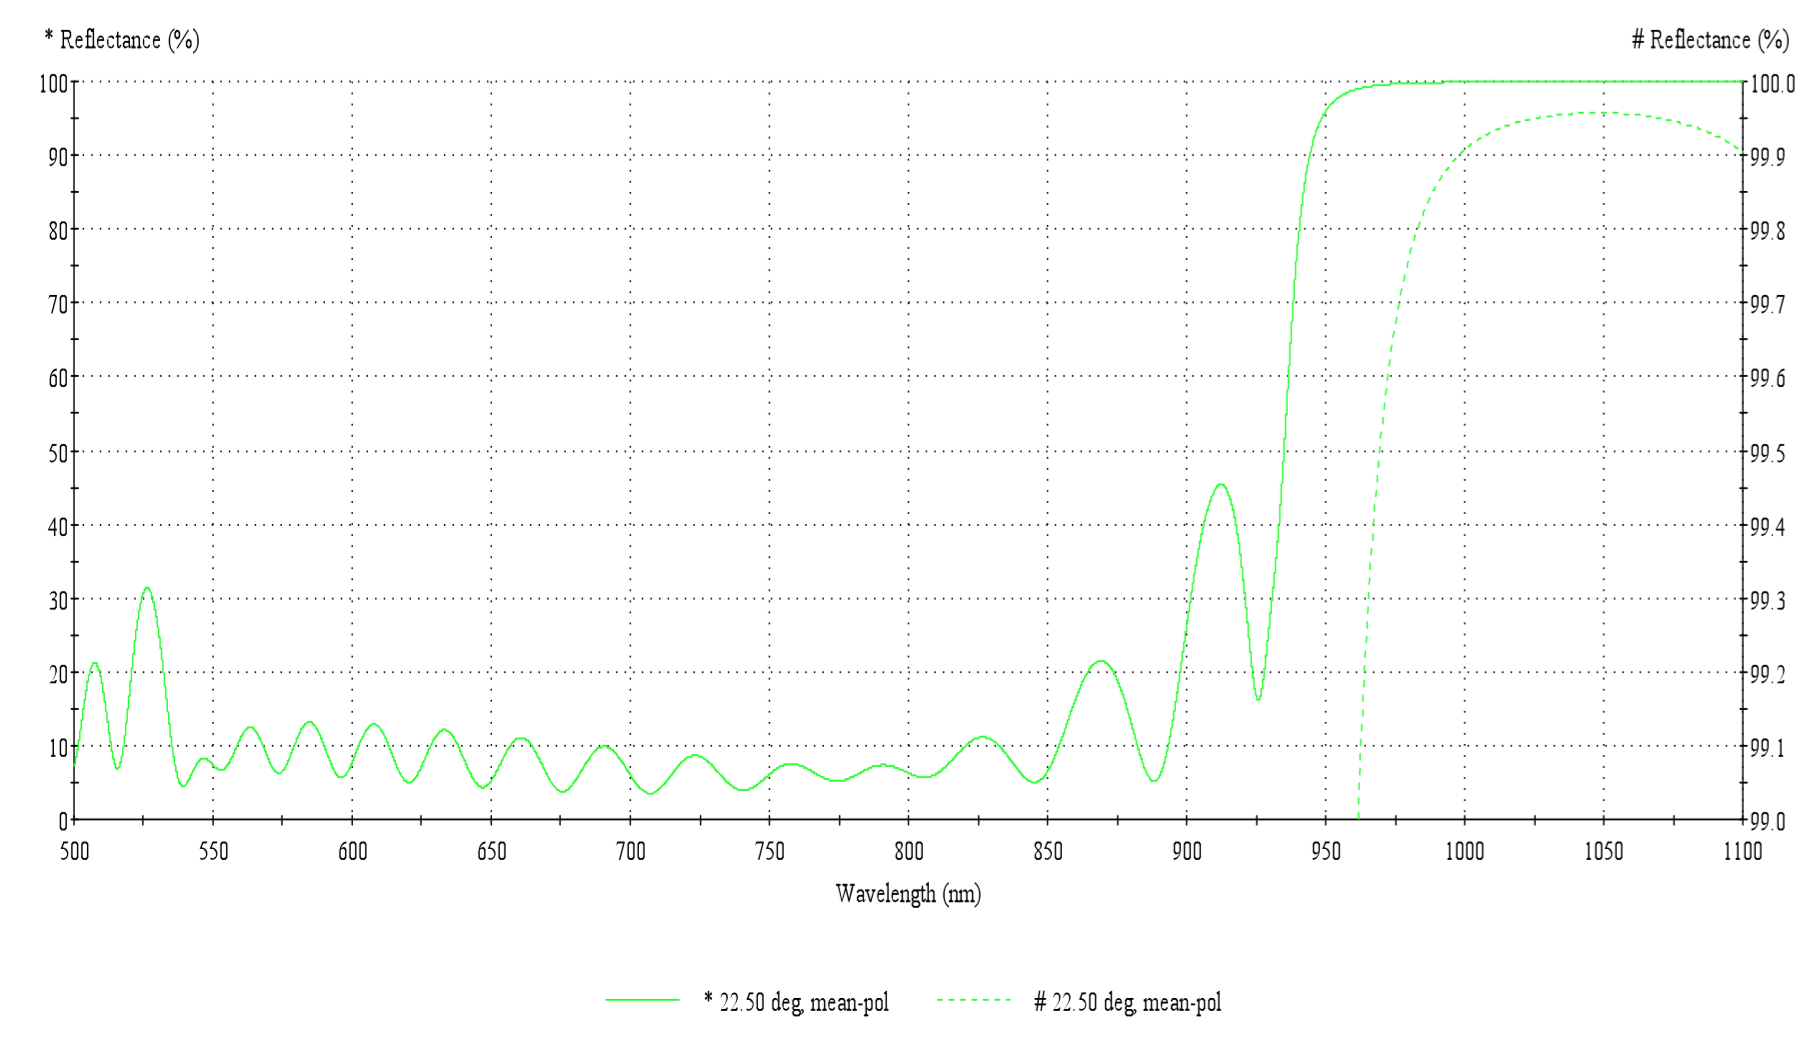
\includegraphics[width=14cm]{Figures/225_HR.eps}
\caption{The simulated HR coating on the fused silica mirror for 22.5 degree of incident angle.  } 
\label{fig:225_HR} 
\end{center}
\end{figure}

\begin{figure}
\begin{center}
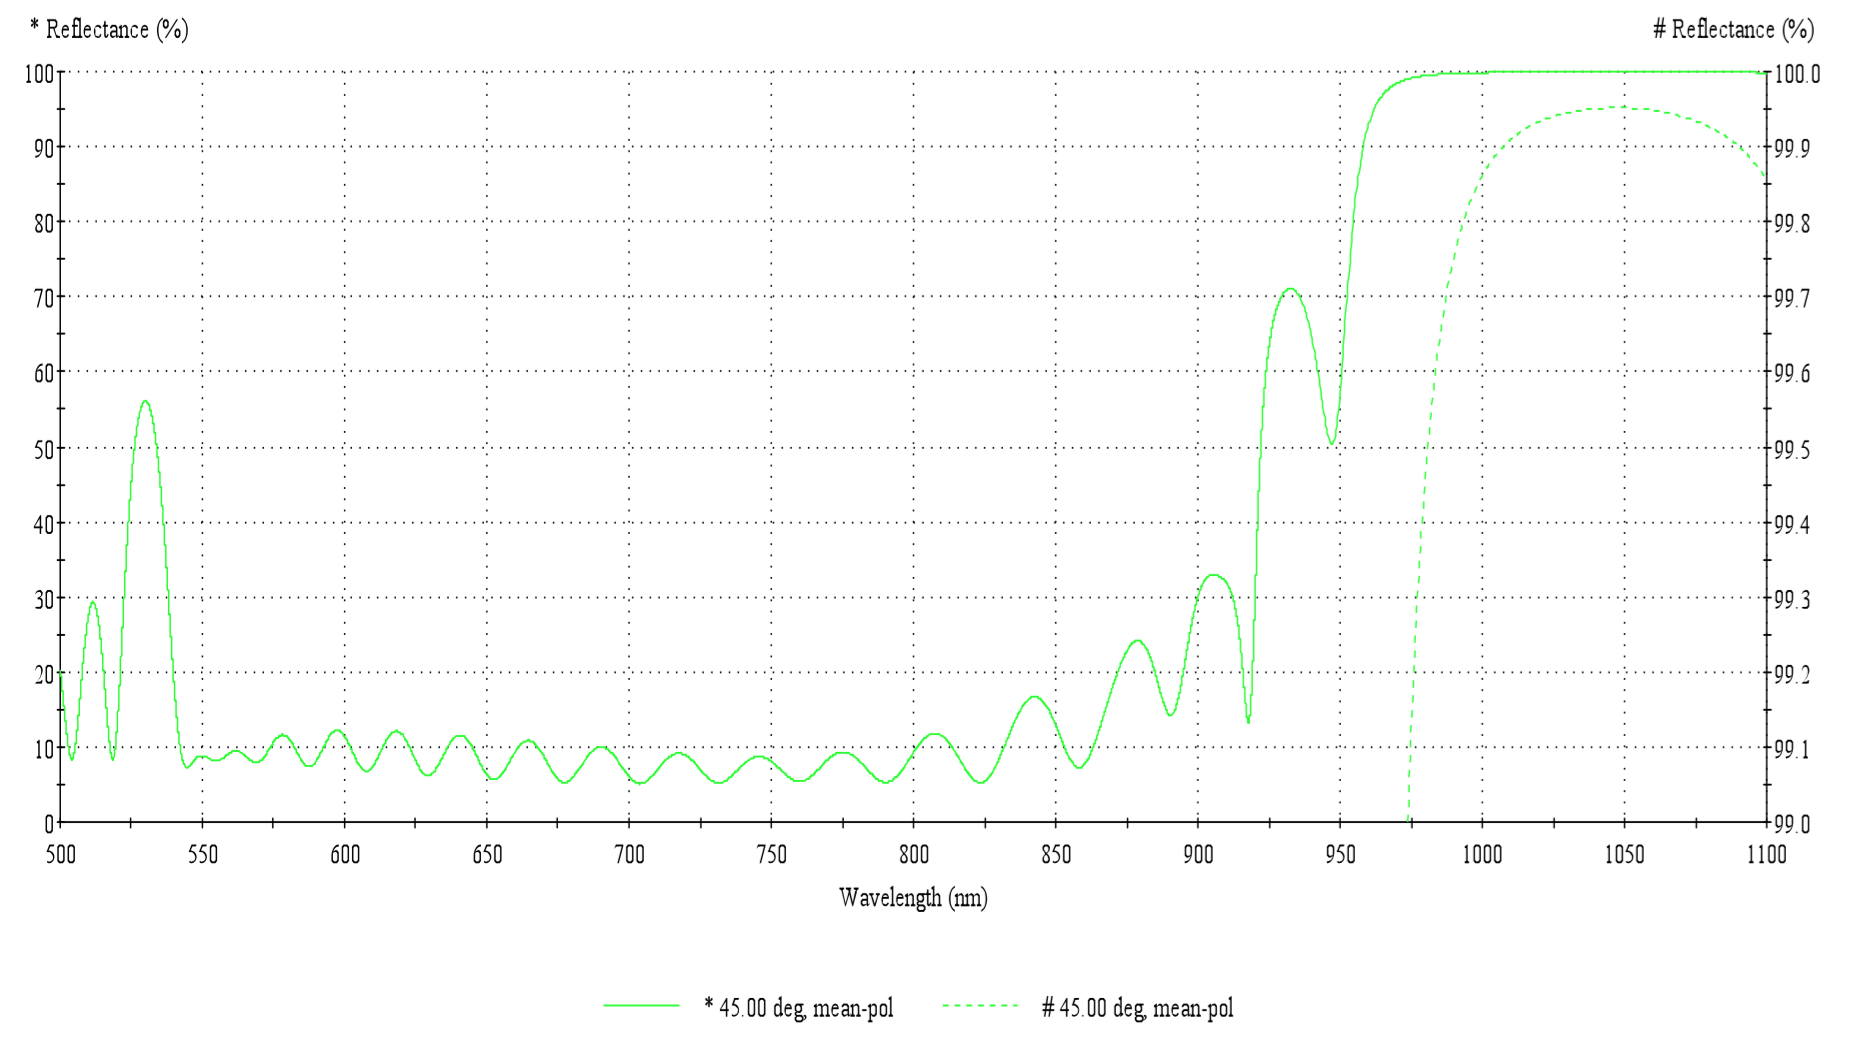
\includegraphics[width=14cm]{Figures/45_HR.eps}
\caption{The simulated HR coating on the fused silica mirror for 45 degree of incident angle. } 
\label{fig:45_HR} 
\end{center}
\end{figure}
 
 \begin{table}
\caption{Specification of Mirrors.}
\label{tab:Tx_mirror_spec}
\centering
\begin{tabular}{ cccccc}
\toprule
\tabhead{Mirror number} & \tabhead{part number}& \tabhead{Diameter [mm]}  & \tabhead{Incident angle}  & \tabhead{Polarization}  \\
\midrule
MTx1 &Y1S-1025-45 (CVI) &25.4  &45& \\
MTx2 &Y1S-1025-45 (CVI)  &25.4  &45& \\
MTx3 &Y1S-1025-45 (CVI) &25.4   &45& \\
MTx4 &Y1S-1025-45 (CVI)  &25.4   &45& \\
MTx5 &Y1S-1025-45 (CVI)  & 25.4  &45& \\
MTx6 &Y1S-1025-45 (CVI)&25.4  &55& \\
MTx7 &Y1S-1025-45 (CVI) &25.4   &35& \\
MTx8 &Y1S-1025-45 (CVI)&25.4   &45& \\
MTx9 &Y1S-1025-45 (CVI)  &25.4   &45& \\
MTx10 &Sigma-koki  & 50.8&45& \\
MTxU11 &Sigma-koki  &  50.8&45& \\
MTxL11 & Sigma-koki & 50.8 &45& \\
MTxU12 &Sigma-koki  & 50.8 &20.9& \\
MTxL12 & Sigma-koki &  50.8&24.1& \\


\bottomrule\\
\end{tabular}
\end{table}
\subsection{Optical mount with Pico-motor}
The uncertainty of the beam position on the ETM is one of the largest systematic errors.
To control the beam position, we employ the Pico-motor for changing mirror angle (see Fig.~\ref{fig:Tx_module_layout}). 
The pico-motor is made by New port, whose part number is 8822. 

\subsection{Beam splitter}
To reduce the elastic deformation, we separate the beam with the beam splitter made by CVI laser optics for pushing the node points of mirror. The part number of beam splitter is BS1-1064-50-2025-45P. The diameter of the beam splitter is 2 inch. Table~\ref{tab:BS_spec} shows the separation ratio of beam splitter.
\begin{table}
\caption{Specification of beam splitter.}
\label{tab:BS_spec}
\centering
\begin{tabular}{ ccccc}
\toprule
\tabhead{Charactaristic} & \tabhead{Typical value} & \tabhead{Unit} & \tabhead{Note} \\
\midrule

Beamsplitter Type&Laser Line Plate Beamsplitters&&\\
Beamsplitter Shape& Round&&\\
Wavelength Range &800 &nm&\\
Bevel/Chamfer & 0.35 mm $\times$ 45 Degree &&\\
Wedge Angle Tolerance & 5& arcmin &\\
Coating Material & Laser Line Dielectric&&\\
Angle of Incidence & 45& Degree&\\
Clear Aperture & 85&\%& \\
Substrate/Material & Fused Silica&&\\
Surface Flatness & $\lambda/10$ &&\\ %% SH Please avoid unicode
Surface Quality & 10-5& scratch-dig& \\
Beamsplitter Diameter & 50.8& mm&\\
Beamsplitter Thickness & 6.35 mm&&\\
Thickness Tolerance &$ \pm0.25~\mathrm{mm}$&&\\
\bottomrule\\
\end{tabular}
\end{table}

\subsection{Optical follower servo}
In order to achieve the low-noise and accurate modulation, an active controller (servo) can modulate the waveform by means of feedback control. This feedback loop used for the Pcal is called as the Optical Follower Servo (OFS).
The OFS will be used in the KAGRA Pcal as a means to reduce the relative power noise (RPN) of the laser. We will achieve maximum sideband to carrier suppression of the modulated output waveform. 
The block diagram of the OFS is shown in Fig.~\ref{fig:OFS_diagram}. The transfer function of this diagram can be described as
\begin{equation}
\frac{AG_1}{1+AKSG_1G_2},
\end{equation}
where A is actuation factor, S is sensing factor, K is percentage of light power sampled, $G_1$ and $G_2$ are gain of feedforward and feedback.

\begin{figure}
\begin{center}
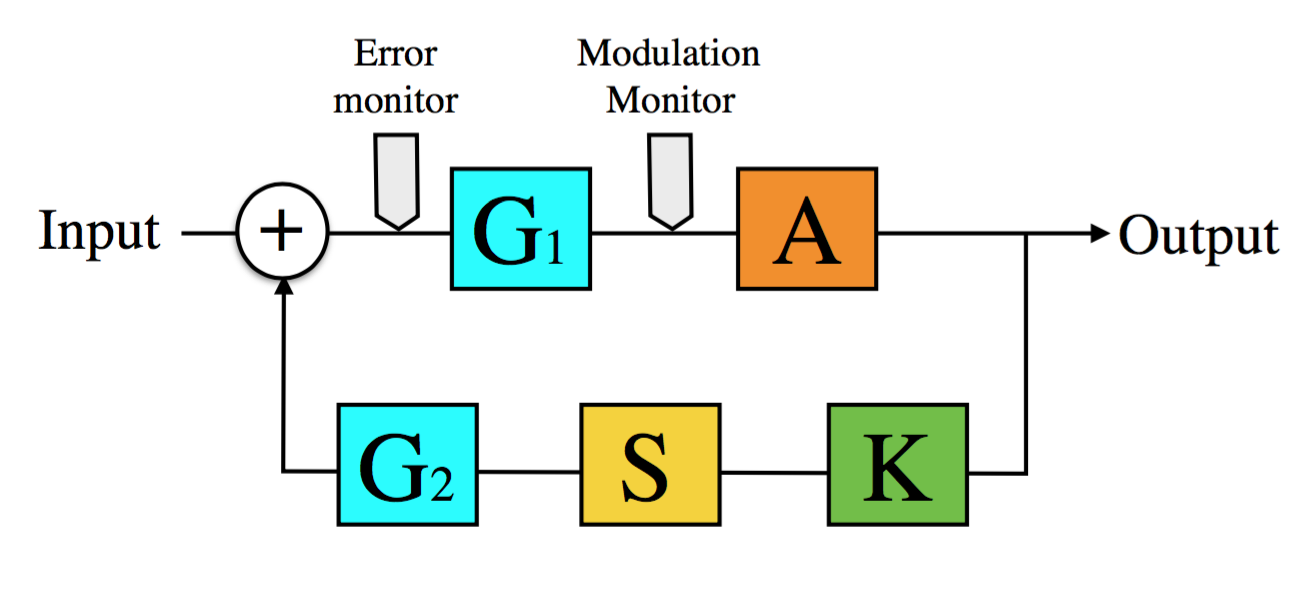
\includegraphics[width=14cm]{Figures/OFS_diagram.eps}
\caption{Diagram of feedback loop for OFS.} 
\label{fig:OFS_diagram} 
\end{center}
\end{figure}


We monitor the difference between test input and \{out1,out2,out3\} .
For monitoring the performance of OFS, we read the location of monitor point.
When we inject the signal, such as swept sine, gauss sine and hardware injection signal, we use input port.
 The estimation of the expected gain parameter is listed in Table.~\ref{tab:OFS_Gain}.

\begin{table}
\caption{Typical gain parameter of OFS. }
\label{tab:OFS_Gain}
\centering
\begin{tabular}{ ccc}
\toprule
\tabhead{} & \tabhead{Gain}& \tabhead{unit} \\
\midrule
A &  0.5 & W/V\\
$G_1$ & 10-100 & V/V(dB) \\
$G_2$ & 2 & V/V(dB) \\
KS &  0.5 & V/W \\
\bottomrule\\
\end{tabular}
\end{table}

The KS corresponds to the trans impedance gain of detector. The detail of photo detector is descrived in Sec.\ref{PD}.
According to Table.~\ref{tab:OFS_Gain}, we regard $G_2KS$ as unity. Therefore, we can simplify the transfer function as follows:
\begin{equation}
\frac{AG_1}{1+AG_1}
\end{equation}
We require the band width of OFS mach larger than operation frequency. We employ the AOM as modulator, which made by ISOMET. The part number of AOM is M1080-T80L-M. The specification is shown in Table~\ref{tab:AOM_spec} 

\begin{table}
\caption{Specification of AOM.}
\label{tab:AOM_spec}
\centering
\begin{tabular}{ ccccc}
\toprule
\tabhead{Charactaristic} & \tabhead{Typical value} & \tabhead{Unit} & \tabhead{Note} \\
\midrule
Spectral Range&$0.36 > 1.5$&$\mu m$&\\
AR Wavelengths& 700 -900 or 1064 & nm &\\
Interaction Medium &Tellurium Dioxide (TeO2)&&\\
Acoustic Velocity & 4.2&$\mathrm{m/\mu s}$&\\
Centre Frequency (Fc) &80& MHz&\\
RF Bandwidth & 30&MHz& \\
Input Impedance&50 &$\Omega$& \\
VSWR&<1.5:1 @ Fc&&\\
Clear Aperture&3.5&mm&\\
Active aperture&1.5&mm&\\
Static Insertion Loss Reflectivity&<3&\%&\\
Laser Polarization&Any&&\\
DC Contrast Ratio&1000:1 min&&\\
Cooling & conduction &&\\
Optical Power&20&W&\\
Beam Diameter&0.5&mm&\\
Optical Rise Time&77&ns&\\
Deflection efficiency & >85 &\%&Pol.: Perpendicular to Base\\
RF power&2.8&W&\@1064nm\\
Bragg angle&10.5&mrad&\@1064nm\\
\bottomrule\\
\end{tabular}
\end{table}

\subsection{Photo detector} \label{PD}
To detect the laser power, we use the photo detector. We place the photodetector at the working standard, Optical follower servo, Integrating sphere in Tx and Rx module.
We developed the photo detector as shown in Fig.~\ref{fig:KAGRA_photodetector}. We employ the InGaAs photo diode for absolute power measurement. The InGaAs diode is placed on the circuit board. The beam is collimated for the power detection reasonably. 

\begin{figure}
\begin{center}
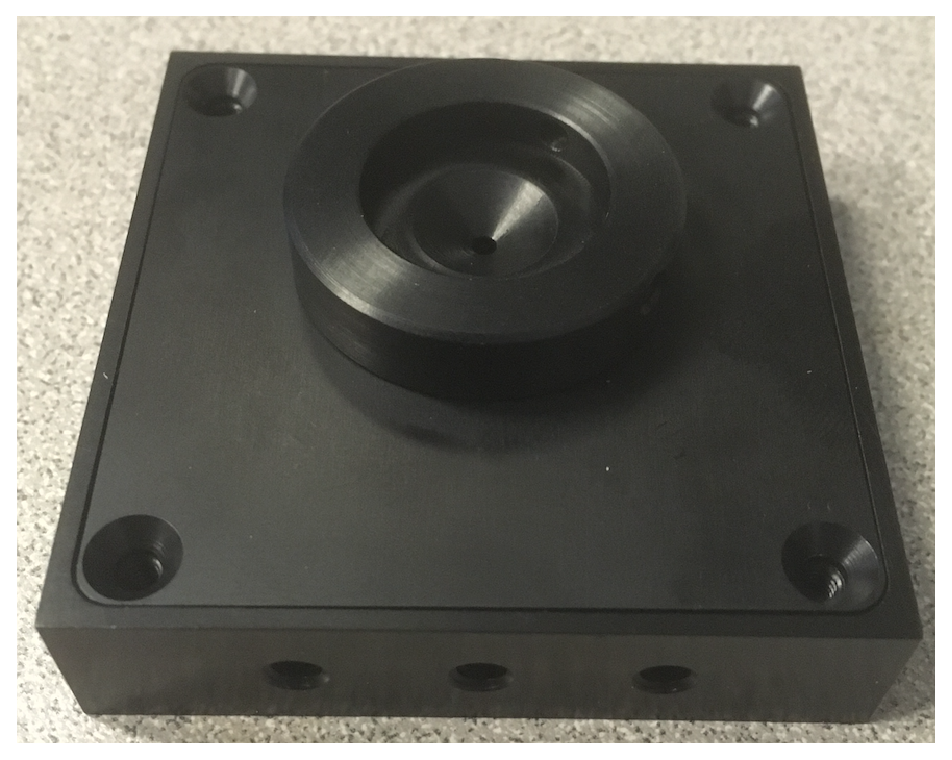
\includegraphics[width=12cm]{Figures/KAGRA_detector.eps}
\caption{Developed photo detector for KAGRA Pcal.} 
\label{fig:KAGRA_photodetector} 
\end{center}
\end{figure}

\subsubsection{Cover}
The cover is designed by the LIGO Pcal group. We make the detector cover in Academia Sinica, Institute of Physics. Figure~\ref{fig:detector_cover} shows the machined detector covers. We housed the circuit board into the cover coated by the black anodized aluminum (MIL-A-8625F, TYPEII,CLASS2). 

\begin{figure}
\begin{center}
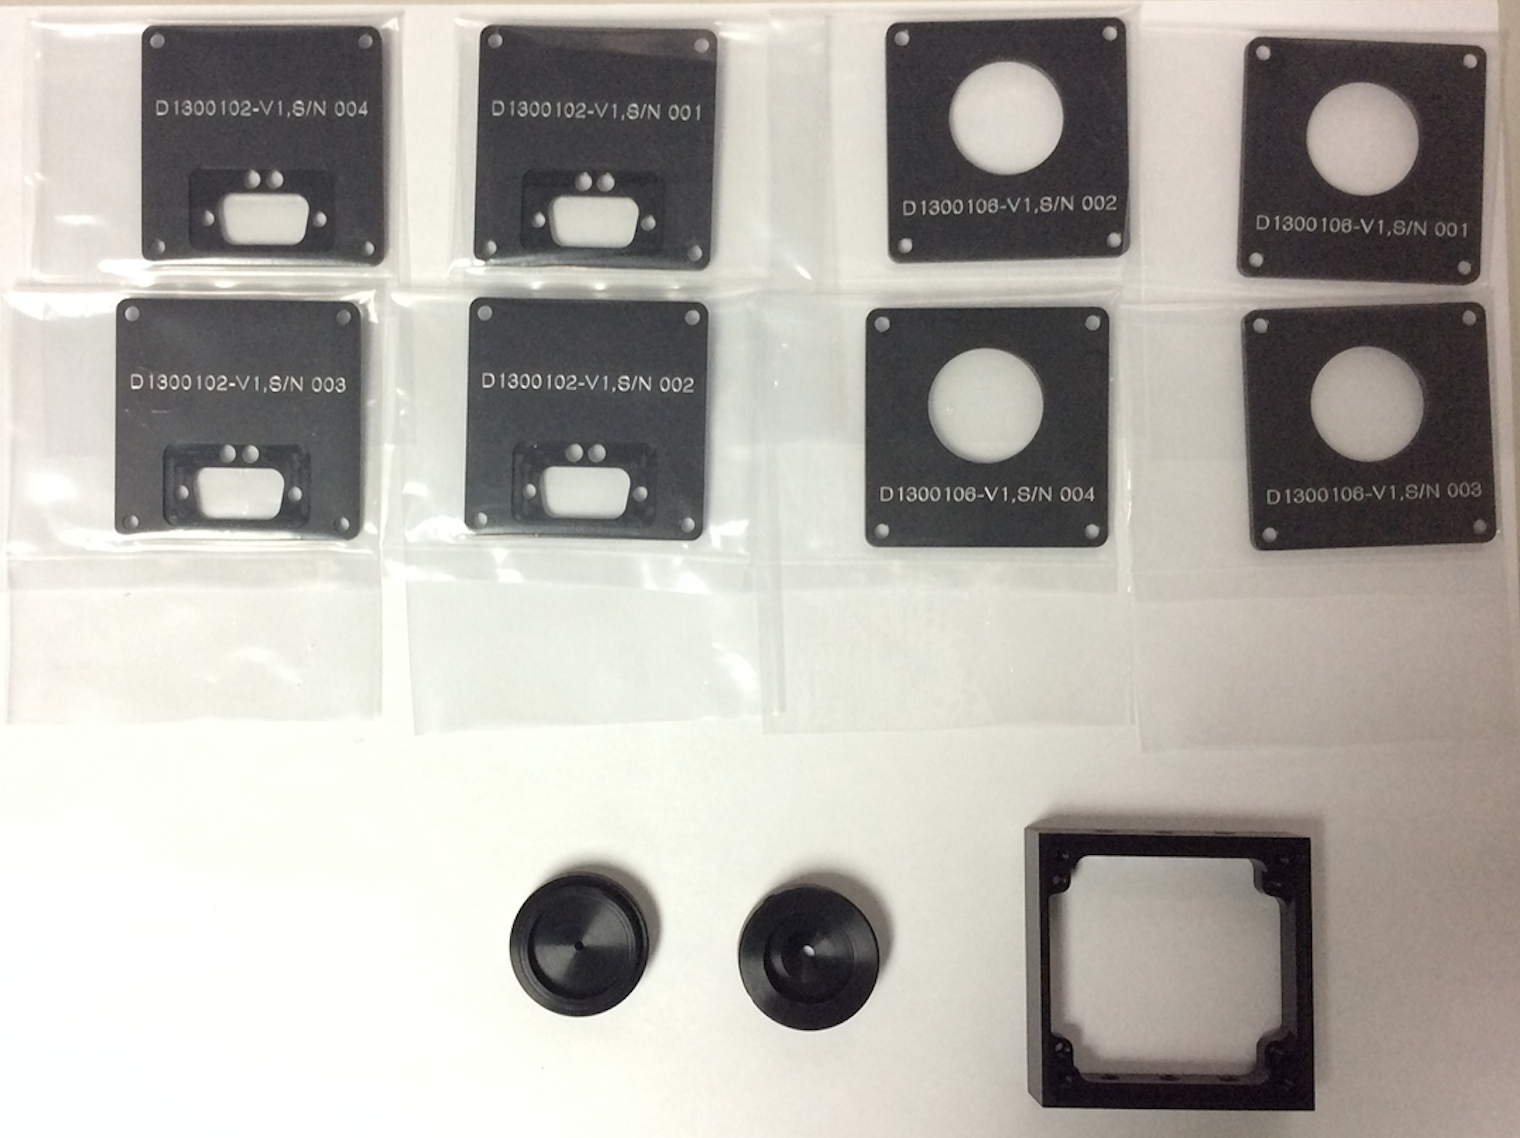
\includegraphics[width=12cm]{Figures/Detector_cover.eps}
\caption{Fabricated cover.} 
\label{fig:detector_cover} 
\end{center}
\end{figure}

\subsubsection{InGaAs detector}	
We employ the C30665GH, which is large area InGaAs PIN photodiode with diameter of 3.0 mm with a flat glass window. The C30665GH provides high quantum efficiency from 800~nm to 1700~nm. This detector is fabricated by Excelitas. The specification of detector is shown in Table.~\ref{tab:detector_spec}.

\begin{table}
\caption{Specification of InGaAs detector.}
\label{tab:detector_spec}
\centering
\begin{tabular}{ ccccc}
\toprule
\tabhead{Charactaristic} & \tabhead{Typical value} & \tabhead{Unit} & \tabhead{Note} \\
\midrule
Dark Current &25& nA& \\
Peak Wavelength&1550& nm& \\
Responsivity&0.95 &A/W&\\
Breakdown Voltage &50 &V& \\
Capacitance & 200 &pF&\\
\bottomrule\\
\end{tabular}
\end{table}


\subsubsection{Electrical Circuit}
We newly improved the electrical circuit of the photon detector as shown in Fig.~\ref{fig:Photo_detector}. The electrical circuit is housed in the aluminum cover. We place the photo detector at the the behind of the electrical circuit. The layers of the circuit consists of 4 layer. We change the differential gain by changing the register and capacitor of the circuit. The electrical circuit are shown in Fig.~\ref{fig:Detector_circuit}.
\begin{figure}
\begin{center}
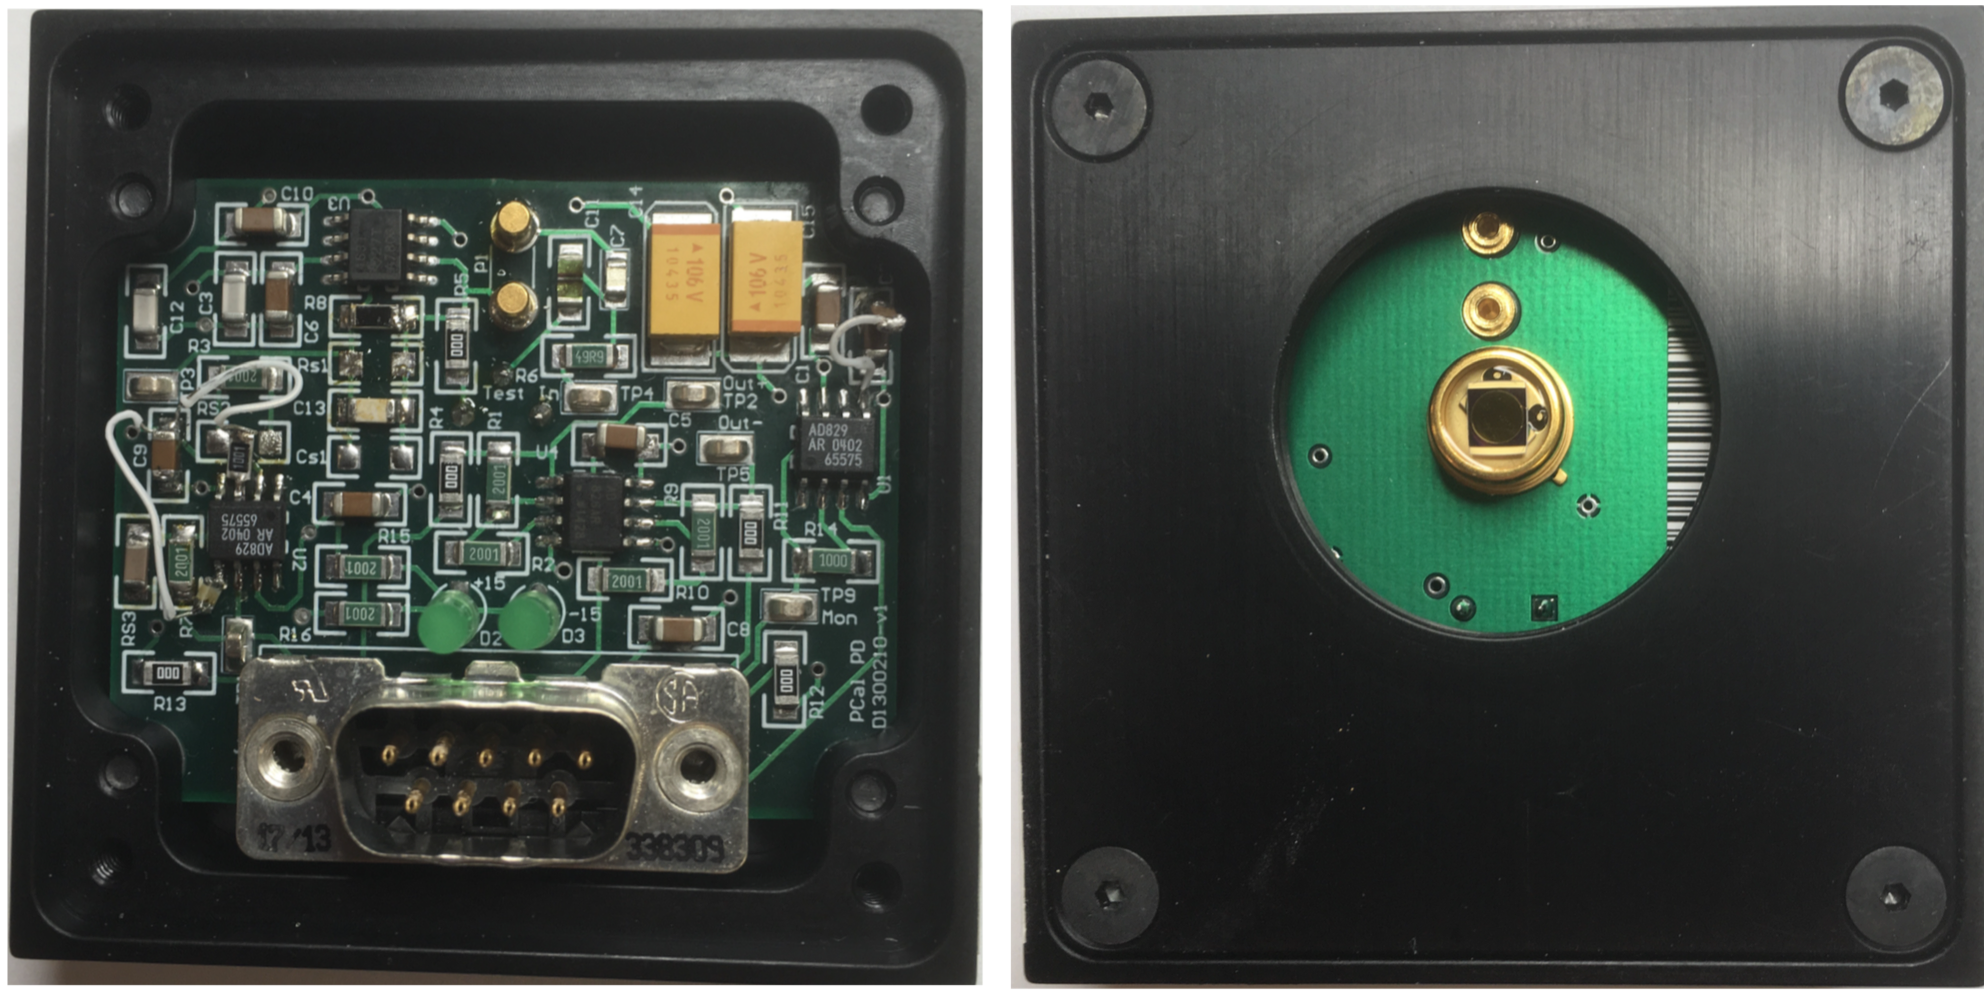
\includegraphics[width=8cm]{Figures/Photo_detector.eps}
\caption{The picture of photo detector. The diameter of photo detector is 3~mm. We control the incident power by changing diameter of the collimator and resistance of trans impedance amplifier} 
\label{fig:Photo_detector} 
\end{center}
\end{figure}
\begin{figure}
\begin{center}
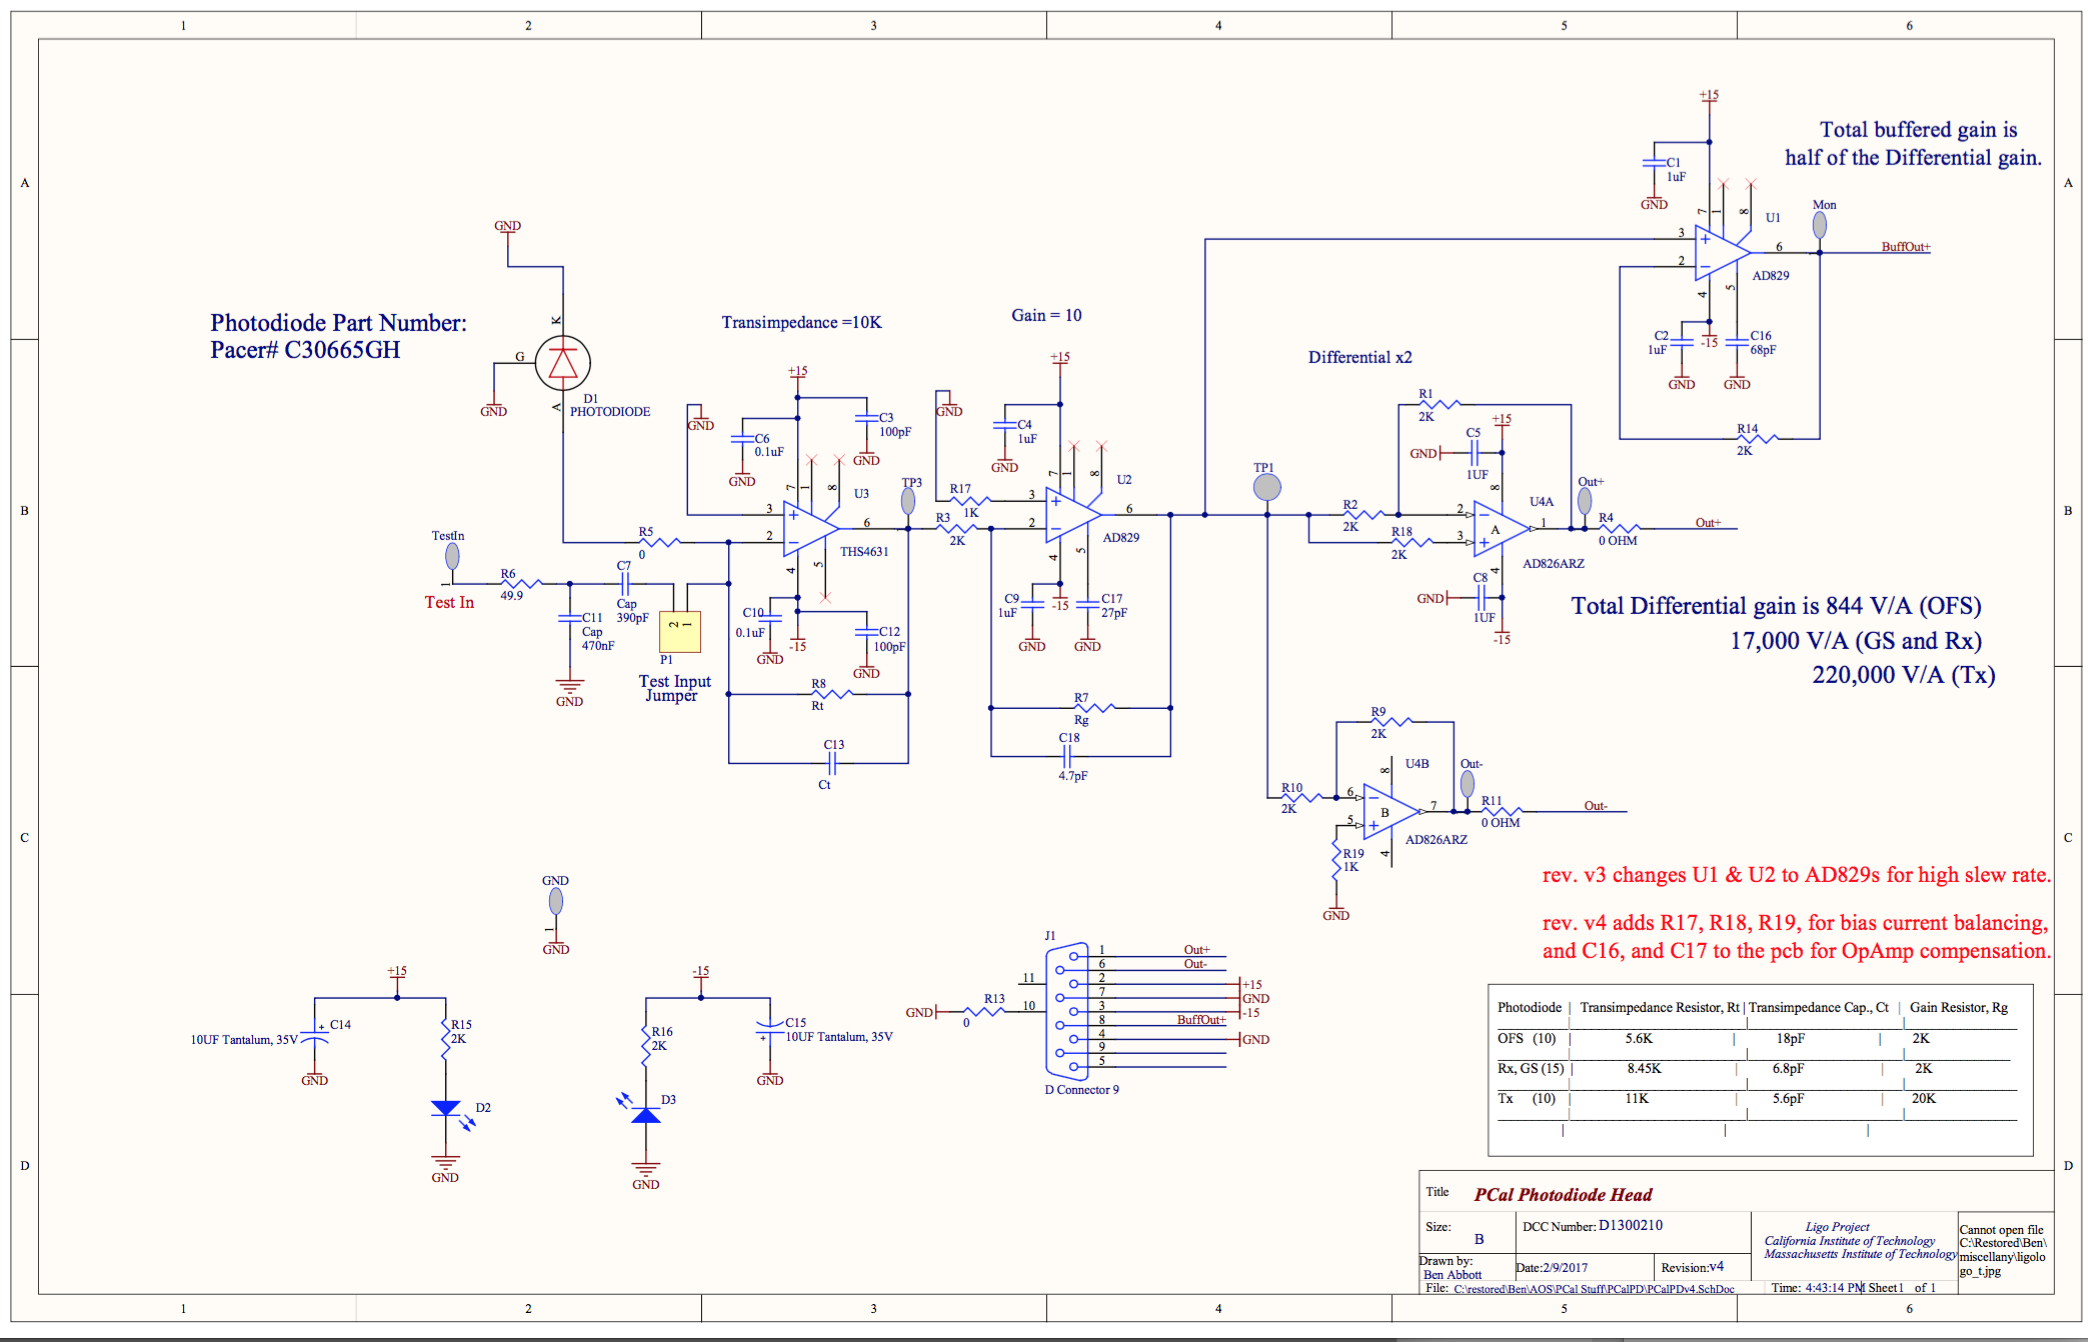
\includegraphics[width=15cm]{Figures/Detector_circuit.eps}
\caption{Circuit of photo detector designed by LIGO (D1300210-v4).} 
\label{fig:Detector_circuit} 
\end{center}
\end{figure}

\subsection{Beam sampler}
Diffractive beam samplers are used to monitor high power lasers where optical losses and wavefront distortions of the transmitted beam need to be kept to a minimum.
In most applications, most of the incident light must to continue forward, "unaffected," in the "zero order" while a small amount of the beam is diffracted into a higher order, providing a "sample" of the beam.
By directing the sampled light in the higher order(s) onto a detector, it is possible to monitor, in real time, not only the power levels of a laser beam, but also its profile.

The operational principle is quite straightforward. From a collimated input beam, the output beams exit from Diffractive Optical Element (DOE) with a separation angle that is determined during the design of the DOE based on the customer's system requirements (See figure 1 below). The separation angle is highly accurate (<0.03mR error). The beams' separation is designed for far-field so that as the beams continue to propagate after DOE, they become more well-defined.
Normally, the customer wishes to get well-focused spots at a certain distance. This is easily achieved by the addition of a simple focusing lens after the DOE, whose BFL (back focal length) determines the working distance (WD) to the multi-spot focal plane.
A Diffractive Beam Sampler allows the high power beam (zero order) to propagate along the optical axis, but produces two side beams with low energy. These two sample beams are located to the left and right of the main beam (-1 and +1 orders), and are characterized by a given separation angle between them and by a given sample power ratio requested by customer. The separation angle is twice the sampled angle.

\subsection{2 inch integrating sphere}
The 2 inches integrating sphere is used for the absolute power measurement of the laser. We receive the separated laser beam at beam sampler. We mount the photo detector (TxPD) at the port of integrating sphere. The integrating sphere is made by the Lab sphere. The inner surface of the integrating sphere in mounted on the Spectralon. The measurement of the absolute power is described in Chep.~\ref{Chapter5}

\subsection{Structure}
The breadboard is placed on the support structure. The material of this structure is SUS 306. This structure can be housed electrical devices, such as driver of the fiber laser, electronics of optical follower servo, and driver of laser shutter. 
%We simulated the resonance frequency using ANSYS. Then, we fix the foot of stracture. The estimated frequency is XXX Hz.

%----------------------------------------------------------------------------------------
\section{Periscope}
The periscope is used for sending the beams to the ETM. We place the periscopes in EXA/EYA chamber as shown in Fig.~\ref{fig:Periscope_overview}.
They consist of four periscopes. The first periscope is mounted at the vacuum side of the window. The laser is sent to second periscope on optical table. We share one first mirror and one second mirror for the two beams of the laser. We send the two laser to two third periscope. The third periscope is sent to fourth periscope, which is aligned to same hight of the injected beam to the ETM. 

\begin{figure}
\begin{center}
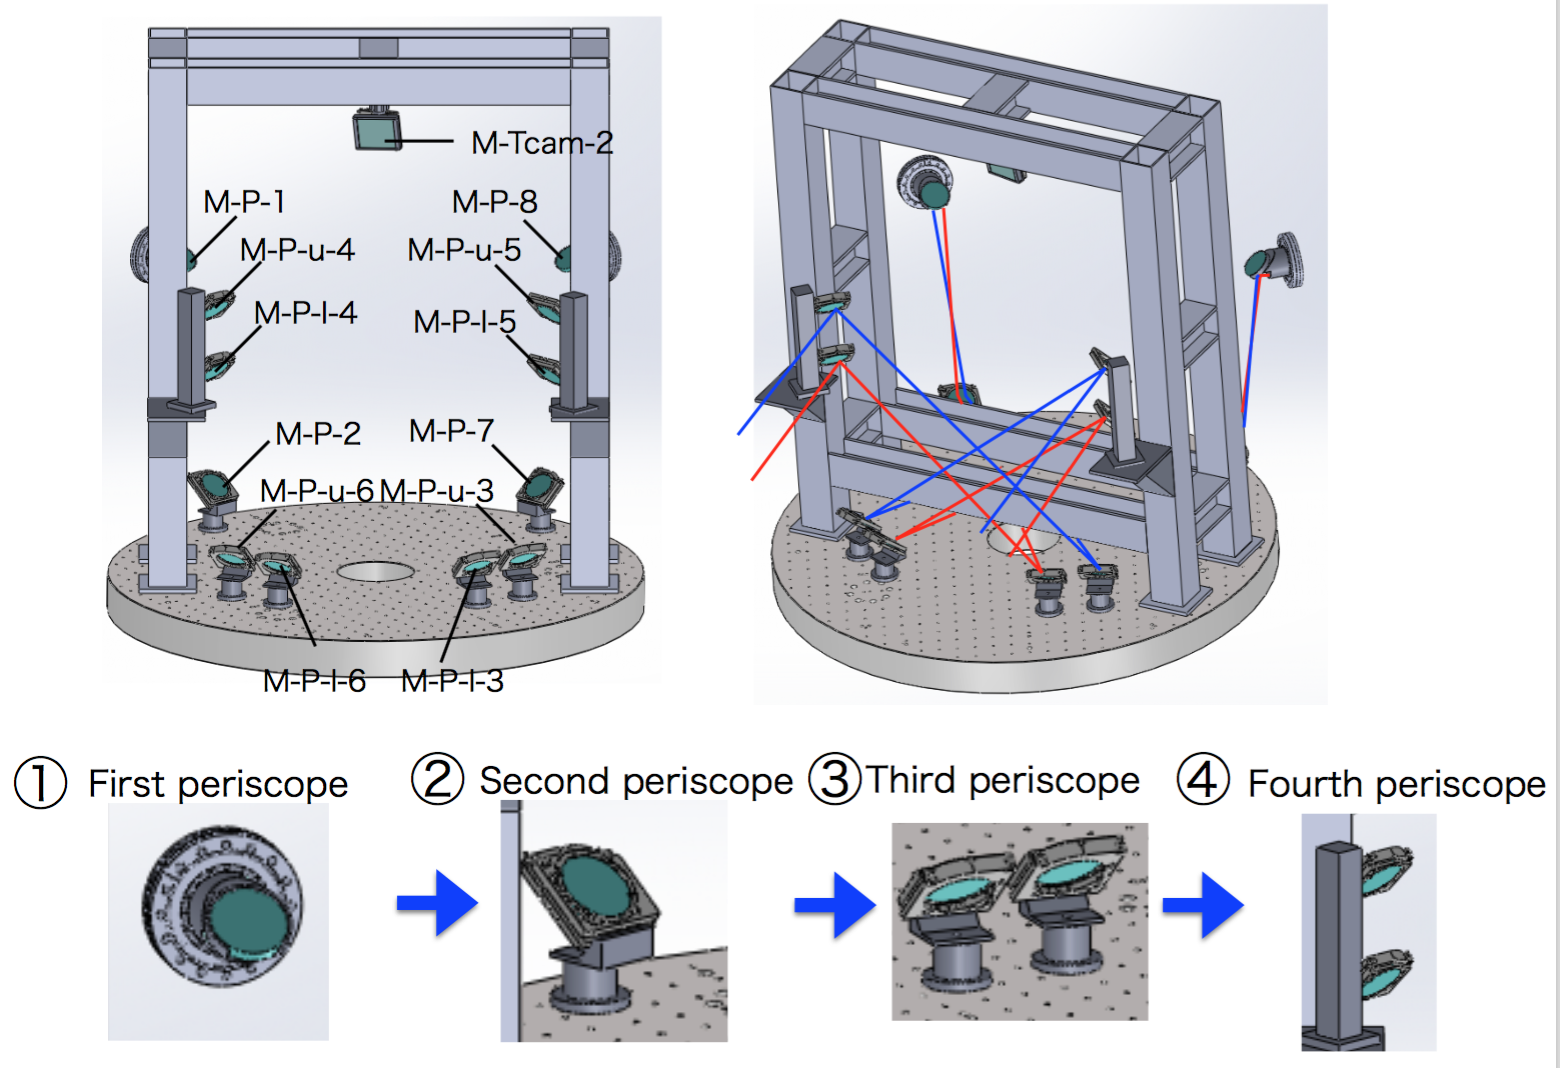
\includegraphics[width=15cm]{Figures/Periscope_overview.eps}
\caption{Periscope structure. We place the twelve 3-inch mirrors in total. The red and blue line correspond to lower and upper beam path, respectively. The upper and lower beams push the node point of the mirror surface.} 
\label{fig:Periscope_overview} 
\end{center}
\end{figure}

\subsection{Geometric optics}
We consider the beam separation and focus position of the beams through the optical component. We fixed 80~mm separation of the mirror in transmitter module.  Figure~\ref{fig:Kikakougaku_position} shows the schematic view of optical layout, where $D_{win}$, $D_{m2}$, and $D_{m3}$ are separation of beams, $L_{win}$, $L_{m2}$, and $L_{m3}$ are distance of each components.  We calculated the beam separation of the vacuum window, second mirror, and third mirrors by changing the focus point as shown in Fig.~\ref{fig:Kikakougaku}. X axis shows the distance from the window. We find a optimal point of minimum separation of the window because of clear aperture of window and second mirror. The optimal focus point is at 355 mm from the window corresponding to 108~mm separation of the mirror. We also find a incident angle of window with optimal focus point as 1.6 degree.




\begin{figure}
\begin{center}
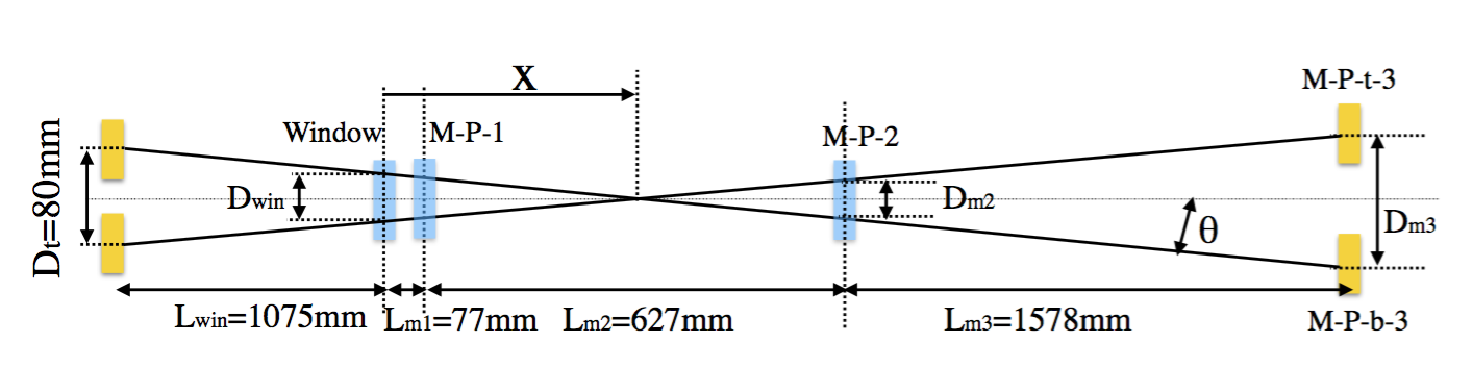
\includegraphics[width=15cm]{Figures/Kikakougaku_position.eps}
\caption{Schematic view of periscope position. We optimized the periscope positions. We fix the separation of Tx module mirror, and each distance, $L_{win}, L_{m1},L_{m2}$ and $L_{m3}$. $x$ is distance from the window.} 
\label{fig:Kikakougaku_position} 
\end{center}
\end{figure}
\begin{figure}
\begin{center}
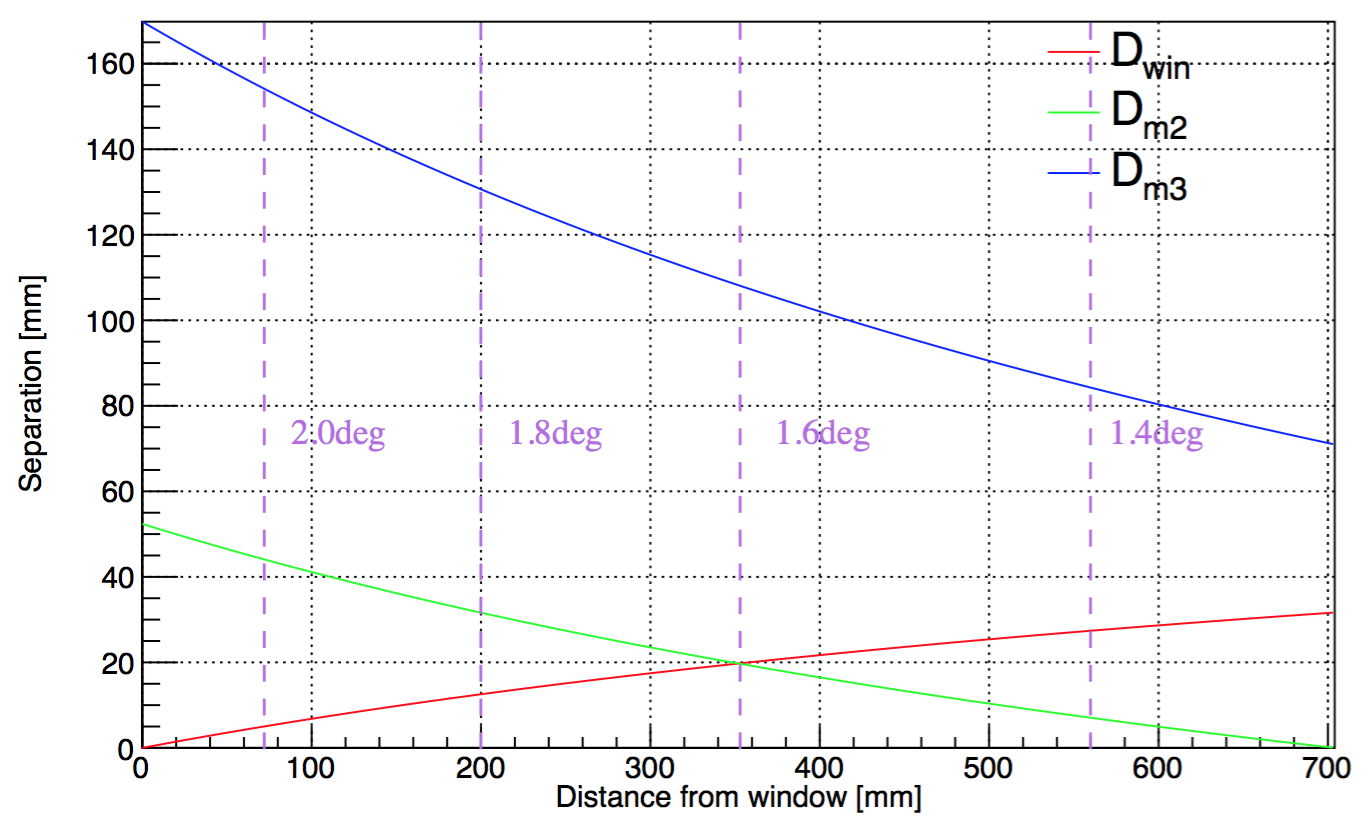
\includegraphics[width=15cm]{Figures/Kikakougaku.eps}
\caption{Calculated separation of $D_{win}$, $D_{m2}$, and $D_{m3}$ by changing the distance from the window. Blue, Green and Red curves are separation position on the window, MP2 and MP3. Purple dashed lines are incident angle of the laser to window. We find the optimal point at 355 mm point corresponding to 1.6 degree incident angle.} 
\label{fig:Kikakougaku} 
\end{center}
\end{figure}

\subsection{View port window}
One of the serious systematic errors are optical efficiency of the view port. Therefore, we have to reduce the reflectance of  view port at least 0.1 \% below. We employ the fused silica optical window whose diameter and thickness are 100 mm and 0.5 inch. We place the AR coating on both surfaces of the window. Figure~\ref{fig:Pcal_win_0} shows the simulated transmittance of the view port. The clear aperture of the view port is about 3 inch. The incident angle of the beams are 1.6 degree. We mounted the first periscope at the vacuum side of the window because we should avoid optical lever path. We set the incident angle of the periscope mirror as 50 degrees.

\begin{figure}
\begin{center}
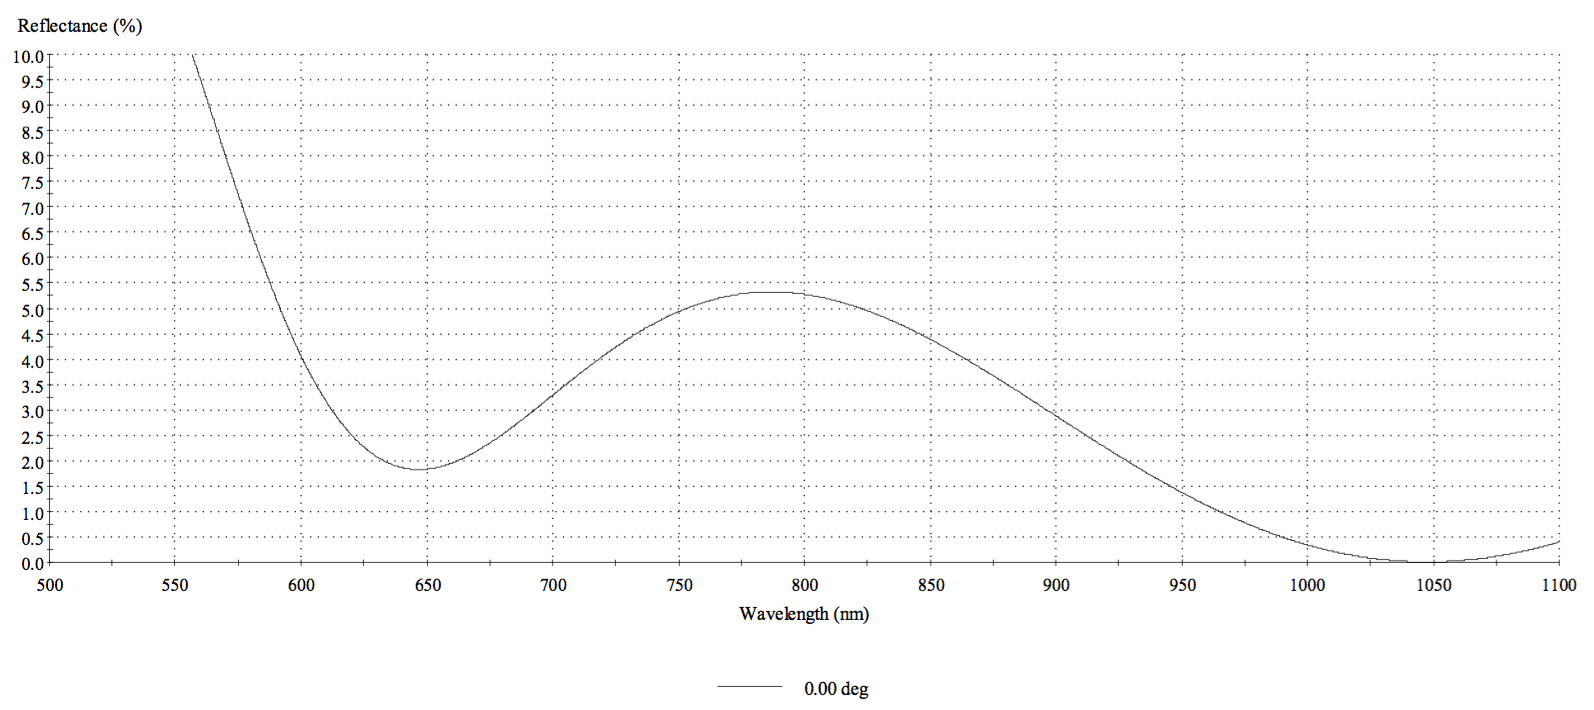
\includegraphics[width=15cm]{Figures/Pcal_win_0.eps}
\caption{Simulated reflection of AR coating of one surface. We optimize the coating frequency at 1047 nm. This plot is provided by Sigma-koki.} 
\label{fig:Pcal_win_0} 
\end{center}
\end{figure}

\begin{figure}
\begin{center}
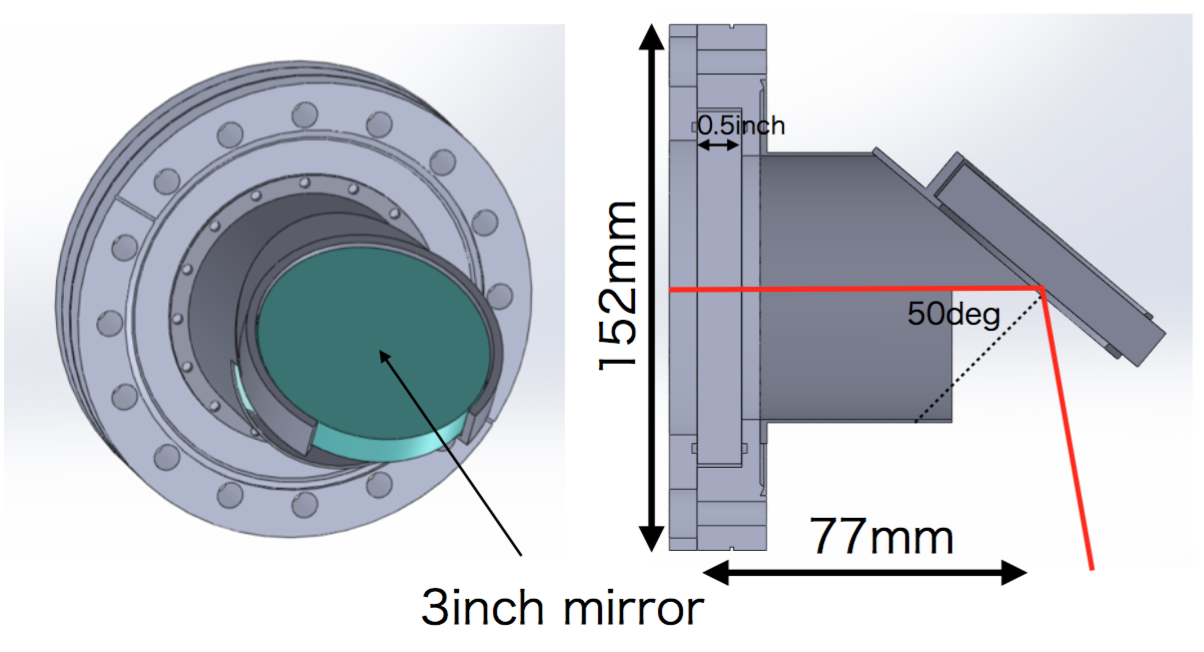
\includegraphics[width=12cm]{Figures/Periscope_window.eps}
\caption{View window with periscope. We mount the AR coated fused silica window on  the ICF152 flange. The AR coating is optimized at 1047~nm. We mount the periscope at the vacuum side of the window. The incident angle of the periscope is 50 degrees.} 
\label{fig:Pcal_window} 
\end{center}
\end{figure}

The flange type of the view port is ICF152. We remodeled the blank flange of ICF 152 made by Cosmotech. Figure ~\ref{fig:Pcal_window} shows the drawing of the view port. We employ the G-85 o-ring for vacuum sealing. 
We have simulated the deformation of window using ANSYS. The assumed Young's module, Poison ratio and density are listed in Table~\ref{tab:ANSYS_win}. The deformation of the window center is $0.85~\mathrm{\mu m}$.

\begin{figure}
\begin{center}
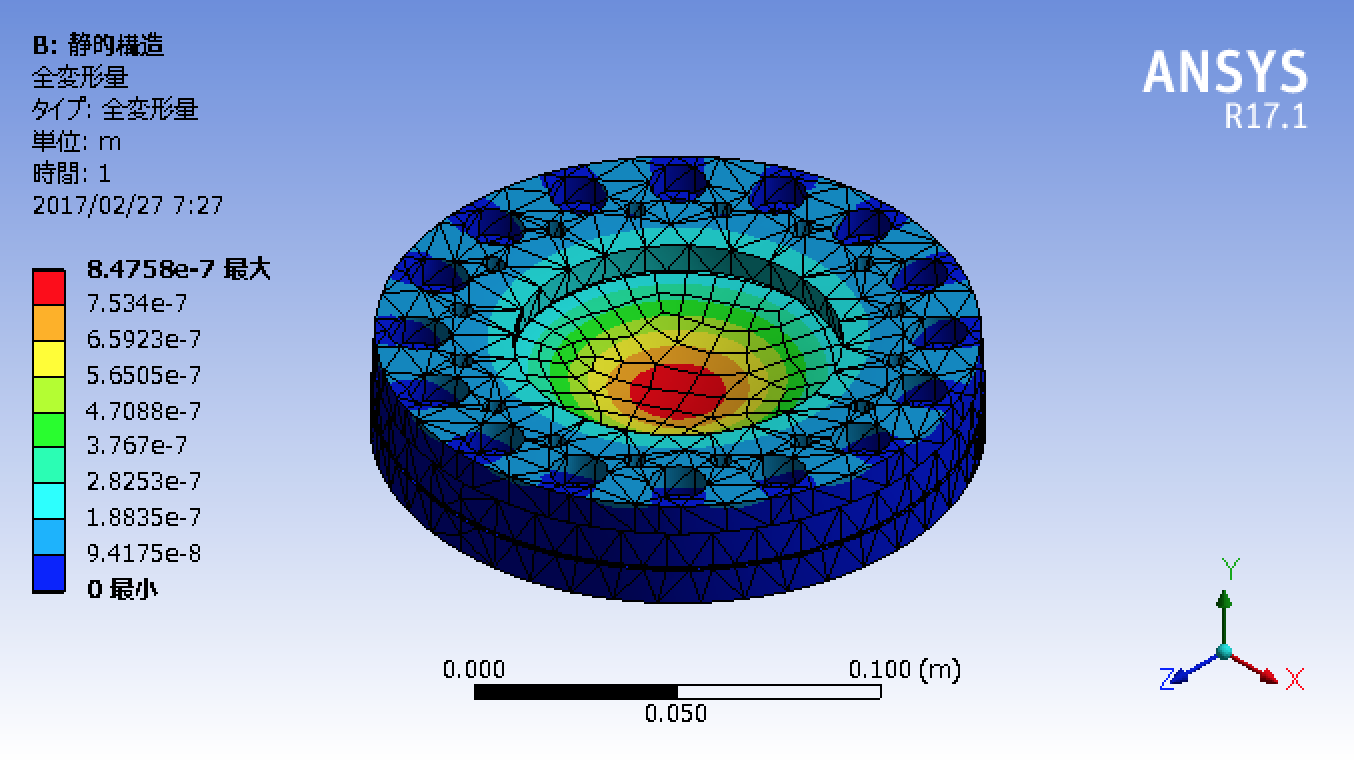
\includegraphics[width=12cm]{Figures/Ansys_window.eps}
\caption{Simulated deformation of Pcal window. The center deformation is $0.85~\mathrm{\mu m}$.} 
\label{fig:Ansys_window} 
\end{center}
\end{figure}

 \begin{table}
\caption{Simulation parameter for ANSYS}
\label{tab:ANSYS_win}
\centering
\begin{tabular}{ccc}
\toprule
\tabhead{Name} & \tabhead{Fused Silica} &\tabhead{SUS306}  \\
\midrule
Young's module &73 Gpa &193 Gpa\\
Poison ratio &0.17& 00.31\\
Density &$2.201\mathrm{g/cm^3}$& $7.750 \mathrm{g/cm^3}$\\
\bottomrule\\
\end{tabular}
\end{table}

\subsection{Mirrors}
We employ eight 3 inch mirrors. We place the HR coating on the polished fused silica disc. The coating and polishing the fused silica is made by Sigma-koki corporation. The reflectance of the mirror is shown in Fig.~\ref{fig:45_HR} and \ref{fig:225_HR}.
 The reflectance of HR coating depends on the incident angle and the polarization angle. The specification of mirrors are summarized in Table.~\ref{tab:Periscope_mirror_spec}. 
 %All mirror is aligned with optical mirror mount made by XXXXXX.
 \begin{table}
\caption{Specification of Mirrors in periscope.}
\label{tab:Periscope_mirror_spec}
\centering
\begin{tabular}{cccccc}
\toprule
\tabhead{Mirror number} & \tabhead{part number}& \tabhead{Diameter [mm]}   & \tabhead{Incident angle}& \tabhead{Polarization}  \\
\midrule
MP1 &  Sigma-koki&76.2  &50.0deg& \\
MP2 &  Sigma-koki &76.2  &50.0deg& \\
MPU3 &  Sigma-koki &76.2   &26.3deg& \\
MPL3 &  Sigma-koki & 76.2  &26.5deg& \\
MPU4 &  Sigma-koki &76.2   &42.9deg& \\
MPL4 &  Sigma-koki &76.2  &41.7deg& \\
MPU5 &  Sigma-koki &76.2   &26.5deg& \\
MPL5 & Sigma-koki & 76.2  &26.3deg& \\
MPU6 & Sigma-koki &76.2   &41.7deg& \\
MPL6 &Sigma-koki  &76.2  &42.9deg& \\
MP7 &Sigma-koki  &76.2  &50.0deg& \\
MP8 & Sigma-koki &76.2   &50.0deg& \\

\bottomrule\\
\end{tabular}
\end{table}


%----------------------------------------------------------------------------------------
\section{Receiver module}
The purpose of the receiver module is to measure the absolute power of laser and beam position control.
All the components are mounted on the optical bench $300 \times 600~\mathrm{mm}$ optical table (B6030L, Tourlabs). 
The optical bench is mounted on the structure.
To accomplish the purpose, we introduce QPD and  6 inch integrating sphere.
The accuracy of beam position and absolute power are corresponding to the systematic errors. 
\begin{figure}
\begin{center}
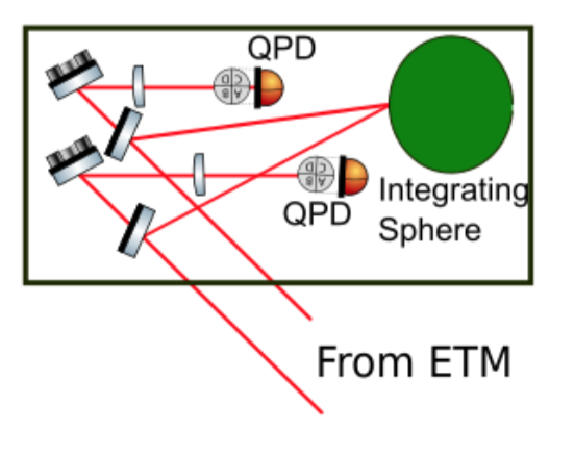
\includegraphics[width=14cm]{Figures/Rx_module_layout.eps}
\caption{Optical layout of receiver module. We mounted QPD for monitoring beam position drift. Total power of the laser is measured by the integrating sphere.} 
\label{fig:Rx_module_layout} 
\end{center}
\end{figure}
\subsection{6 inch Integrating sphere}
The 6 inches integrating sphere is used for absolute power measurement of the laser. We receive the laser beam from two paths. To receive the power perfectly, we need a large diameter hole of integrating sphere at least 2 inch. We use for the 2 inch hole integrating sphere. We mounted the photo detector at the top of port. Details of the photo detector is explained in Sec.~\ref{PD}.

\subsection{Mirror}
We employ four 3 inch mirrors. We place the HR coating made by Siguma-koki as shown in Fig.~\ref{fig:45_HR} and \ref{fig:225_HR}. For two mirrors, we make the AR coating on the back surface to pick up the beams. The specification of the mirrors are listed in Table~\ref{tab:Rx_mirror_spec}.
 \begin{table}
\caption{Specification of Mirrors in Rx module.}
\label{tab:Rx_mirror_spec}
\centering
\begin{tabular}{ cccccc}
\toprule
\tabhead{Mirror number} & \tabhead{part number}& \tabhead{Diameter [mm]} & \tabhead{Incident angle}& \tabhead{Polarization}  \\
\midrule
MRx1 &Sigma-koki&76.2 &21.7deg& \\
MRx2 &Sigma-koki &76.2 &23.3deg& \\
MRx3 &Sigma-koki&76.2   &21.7deg& \\
MRx4 &Sigma-koki&76.2     &23.3deg& \\
\bottomrule\\
\end{tabular}
\end{table}



\subsection{QPD}
We will implement QPDs for beam position control, which made by Tholabs.  They also help us to understand the alignment drifts of the beams. The part number of QPD is PDQ30C as shown in Table.~\ref{tab:detector_spec}.
\begin{table}
\caption{Specification of QPD.}
\label{tab:detector_spec}
\centering
\begin{tabular}{ ccccc}
\toprule
\tabhead{Charactaristic} & \tabhead{Typical value} & \tabhead{Unit} & \tabhead{Note} \\
\midrule
Substrate&	InGaAs&&\\
Wavelength Range&1000 - 1700& nm&\\
Detector Bandwidth	&150 &kHz& \\
Recommended Spot diameter	&$\phi0.2$ - $0.5$ & mm &\\
\bottomrule\\
\end{tabular}
\end{table}

%----------------------------------------------------------------------------------------

\section{Camera module} \label{Tcam_inst}
The beam position of the ETM surface corresponds to systematic error of the rotation and elastic deformation. To measure the beam position, we measure the mirror surface directly. However, the KAGRA EXA/EYA chambers are placed at 36m far from the ETM. Thus, we employ the combination of telescope and high resolution camera, we call telephoto camera (TCam). We are tuning with focus point of the mirror using focuser.  We place the view port and mirror between the ETM and TCam. Figure~\ref{fig:Camera} shows the drawing of TCam unit.

\subsection{Camera}
Purpose of using the high resolution camera, we have to measure the beam position within 1 mm accuracy. Ww solved this problem by D810 digital camera made by Nikon. The D810 reprises the 36-megapixel resolution with $35.9 \times 24.0~\mathrm{mm}$ CMOS sensor. We remove the IR filter because the commercial camera is not sensitive to laser wavelength (1047 nm).

\subsection{Telescope}
We employ the Maksutov-Cassegrain type telescope for observing the ETM surface. The diameter of the primary mirror is 127 mm and its focal length is 1500 mm ($f/12$). The telescope is manufactured by Sky-watcher company. The diameter of the telescope is limited by the that of the view window size. 

\subsection{Focuser}
A focuser, which is made by Moonlight, is used for the automatic focus control. 
We connect focuser between telescope and camera. 
The picture of focuser is show in Fig.~\ref{fig:ML_focus}.
\begin{figure}
\begin{center}
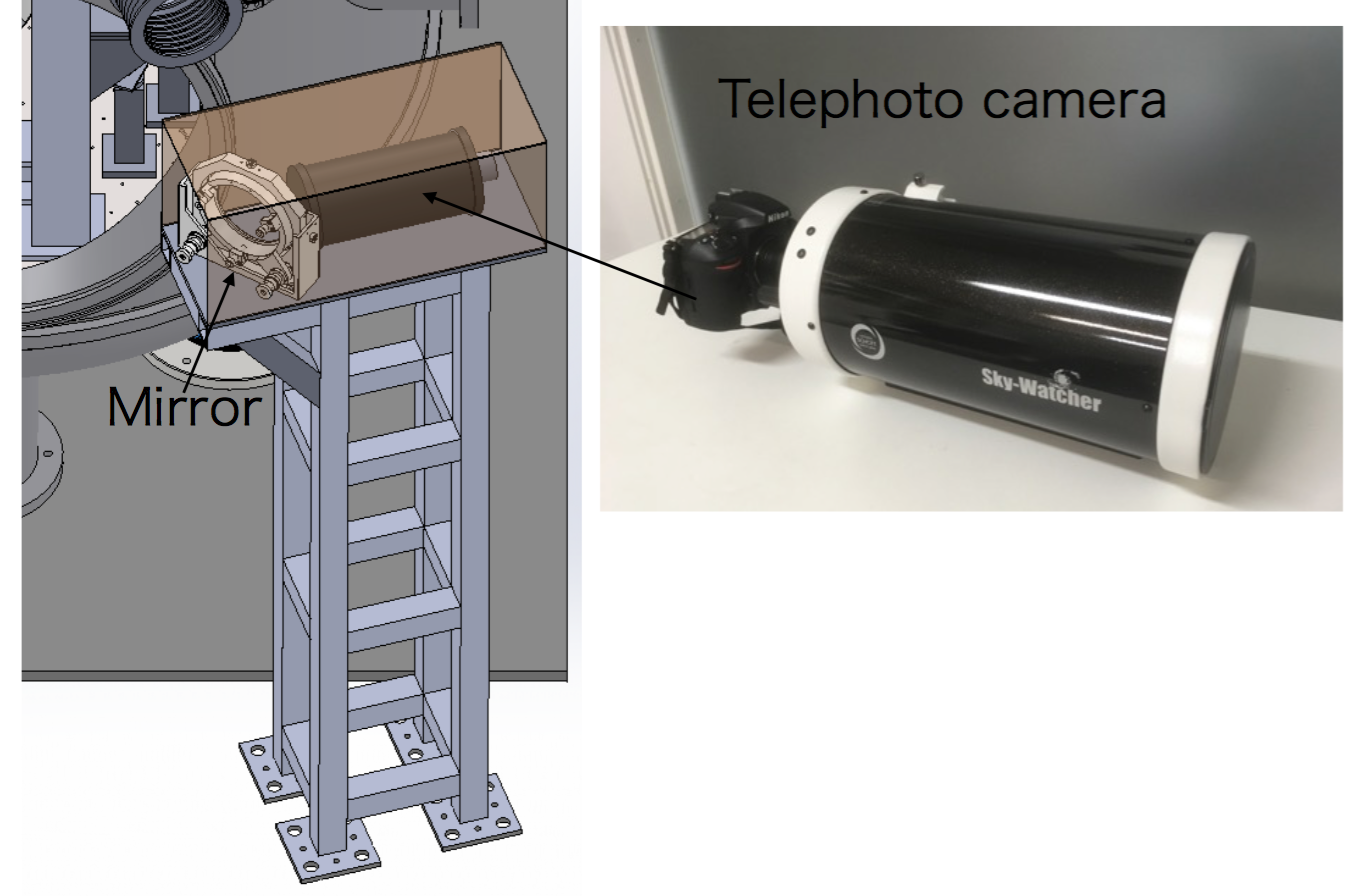
\includegraphics[width=12cm]{Figures/Camera.eps}
\caption{Mirror and Telephoto camera (TCam). We place the TCam on the structure.The image of ETM is referred by two mirrors. One mirror is mounted in vacuums. Another is placed at outside of chamber. The specification of mirrors are listed in Table.~\ref{tab:Camera_mirror_spec}.} 
\label{fig:Camera} 
\end{center}
\end{figure}

\begin{figure}
\begin{center}
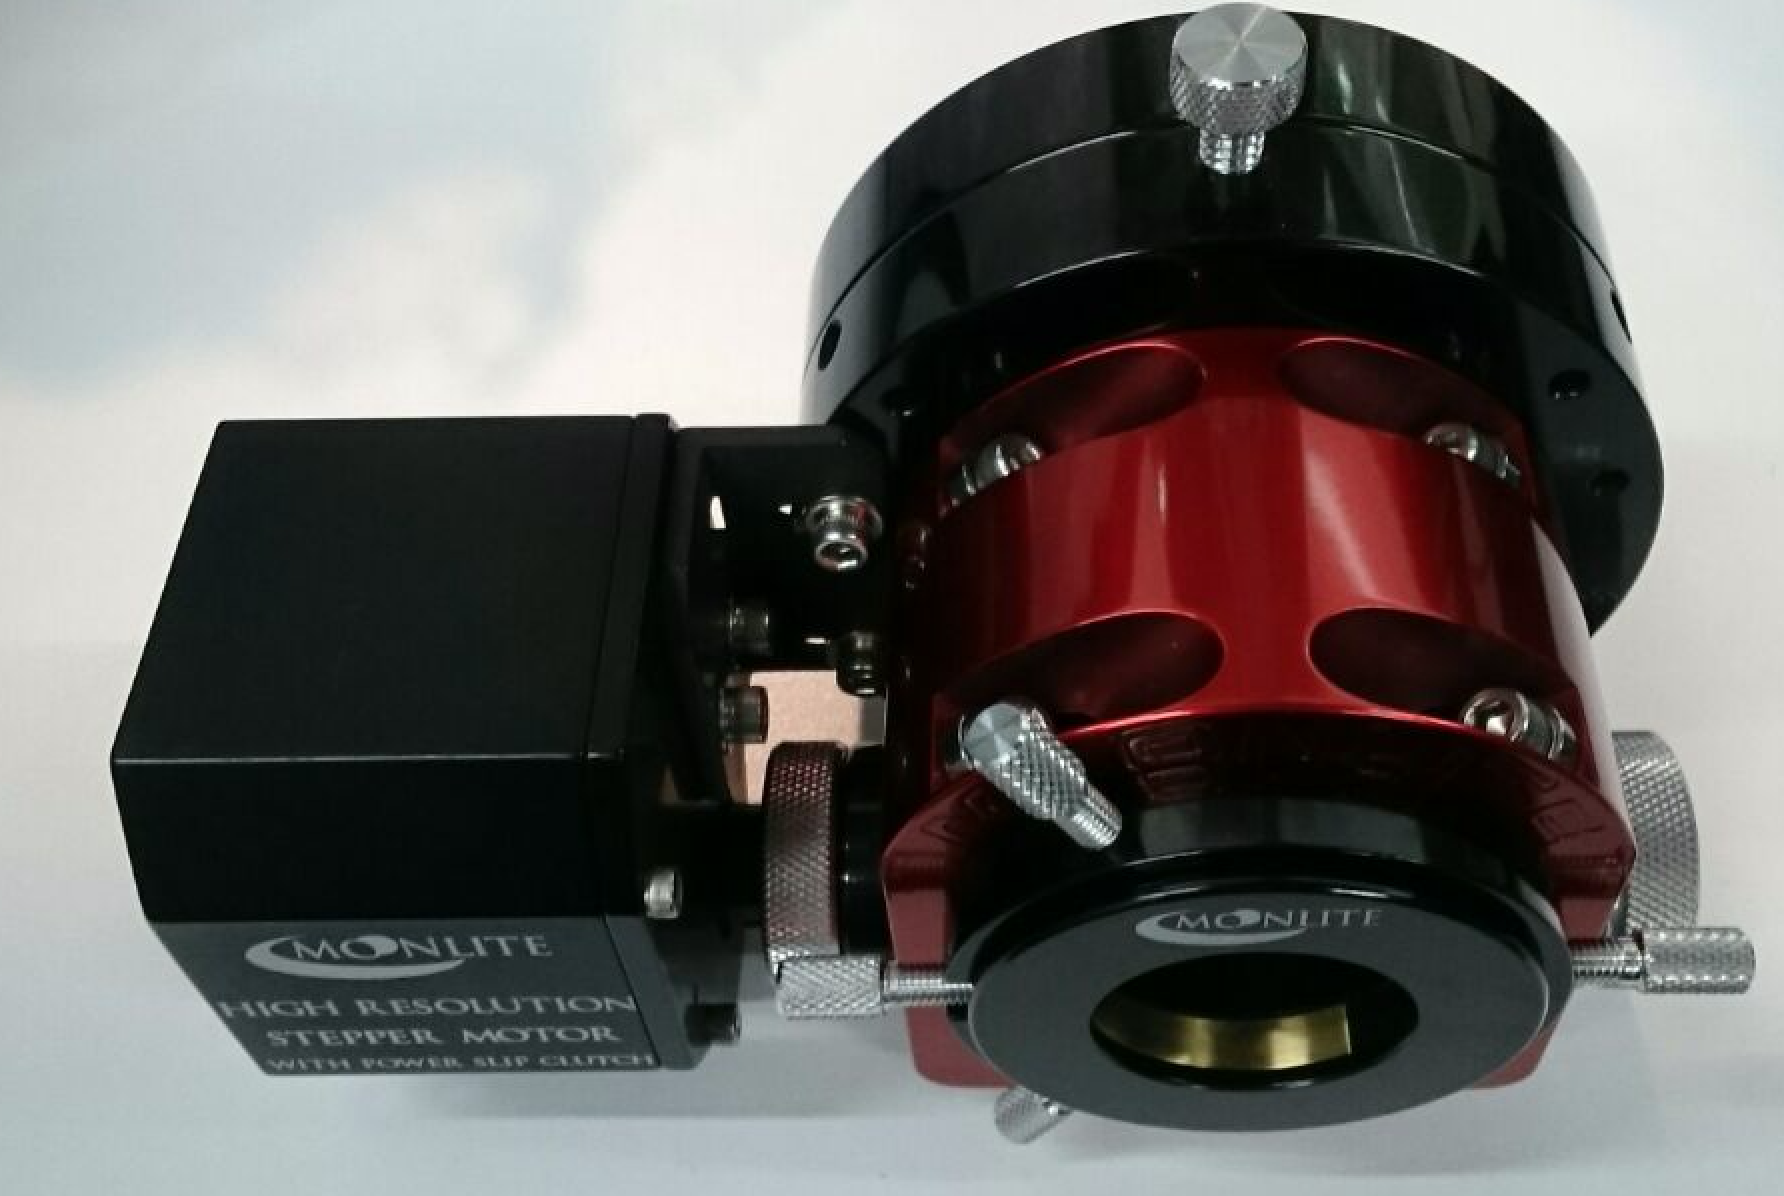
\includegraphics[width=12cm]{Figures/ML_focus.eps}
\caption{Moon light focuser.}
\label{fig:ML_focus} 
\end{center}
\end{figure}


\subsection{View port window}
The flange type of the view port is ICF203. We remodeled the blank flange of ICF 203 made by Cosmotech. Figure~\ref{fig:Camera_window} shows the drawing of the view port. We employ the G-135 o-ring for vacuum sealing. 


 \begin{table}
\caption{Specification of mirrors in camera}
\label{tab:Camera_mirror_spec}
\centering
\begin{tabular}{cccc}
\toprule
\tabhead{Mirror number} & \tabhead{part number}& \tabhead{Size [mm]}   & \tabhead{Incident angle}  \\
\midrule
MTcam1 &TFA-150C20-10 (Siguma-koki)&  $\phi150$  &45deg \\
MTcam2 &TFA-80100R15-10 (Sigma-koki)&  $100 \times 80$  &30 deg \\
\bottomrule\\
\end{tabular}
\end{table}

\begin{figure}
\begin{center}
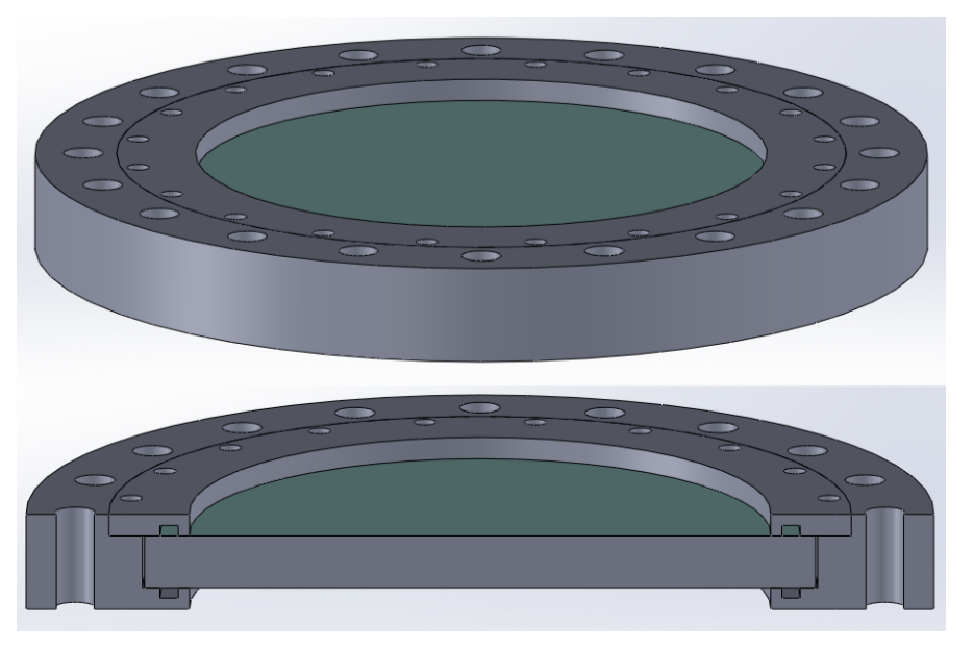
\includegraphics[width=12cm]{Figures/Camera_view_window.eps}
\caption{Window design. We employ the AR coated fused silica window.} 
\label{fig:Camera_window} 
\end{center}
\end{figure}

\subsection{Mirror}
We mount the two mirrors for Tcam. One mirror place in EXA/EYA chambers, whose size is $100 \times 80~\mathrm{mm}$. This mirror is made by Thorlab. another mirror is mounted on the structure of the camera mount, whose diameter is 150~mm. The specification of the mirrors are listed in Table~\ref{tab:Camera_mirror_spec} .


\subsection{Illuminator}
To illuminate the mirror surface for taking picture, we place the illuminator

%----------------------------------------------------------------------------------------
\section{MEDM} \label{MEDM}
All the system are controlled by Epics-MEDM. Figure~\ref{fig:MEDM} shows the prototype MEDM system for KAGRA PCal.
\begin{figure}
\begin{center}
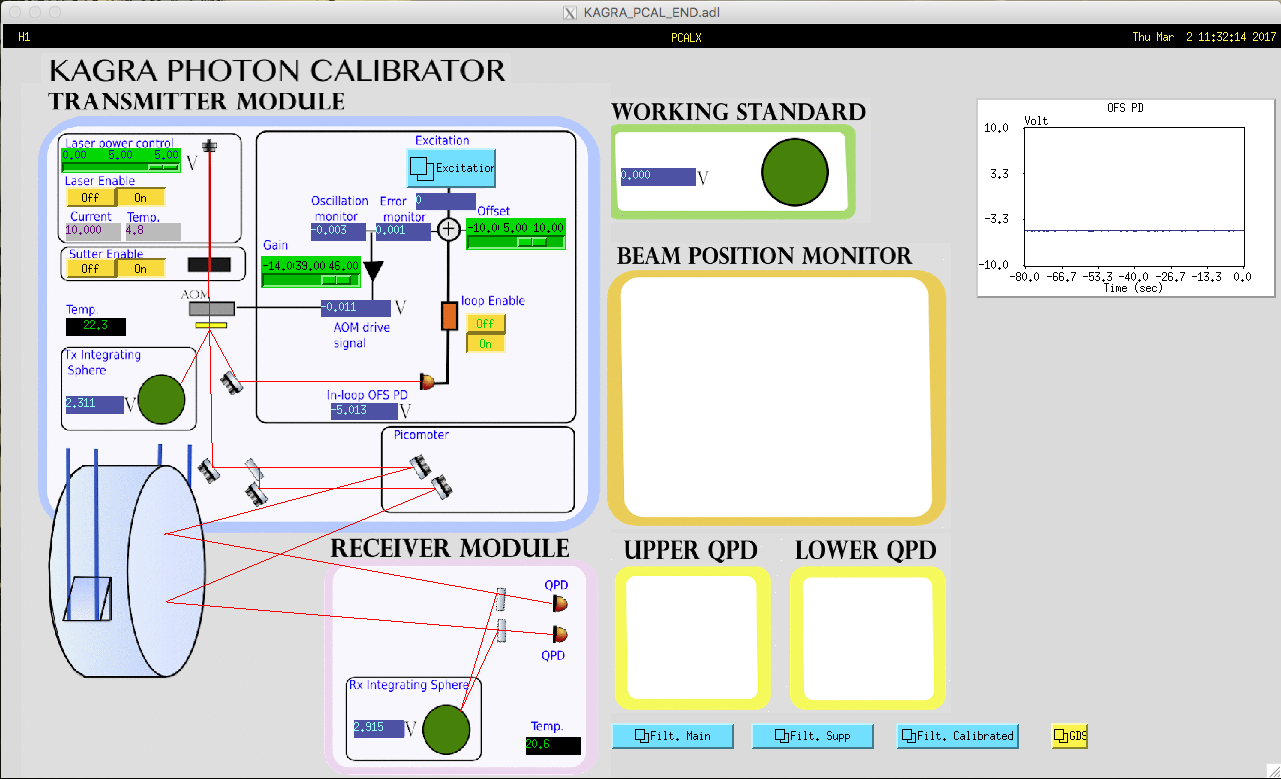
\includegraphics[width=12cm]{Figures/MEDM.eps}
\caption{MEDM of KAGRA photon calibrator. The system is based on LIGO MEDM.We improve this system for BMS.}
\label{fig:MEDM} 
\end{center}
\end{figure}

\section{Summary}
There is a need for future demonstration to better under standing how accurate measurement.
Im particular, we should test the improved performance of high power laser, and  beam position monitoring system (BPM).
Overall, our optimized instrumental design make the essential role of systematic error understanding for KAGRA and other experiment.
The strengths of one design are high power laser, symmetrical optical desgn, and BPM.
These technology make the understand character of IFO easier.
Finally, we show that this novel techniques is a promising tools to generate significant GW data.
